%*******************************************************************************
%****************************** Terzo Capitolo **********************************
%*******************************************************************************
\chapter{Dati e esperimenti}
\label{chapter3}
% ********************************** Sezione 3.1  **************************************
\section{Esperimento 1 - Fix di posa simulato con \texttt{Rviz}}
\label{section3.1}
Nel primo esperimento l'obiettivo è quello di dimostrare la bontà della procedura di fix di posa messa a punto.


Per fare ciò, dopo che l'algoritmo AMCL si è avviato ed il robot si è correttamente localizzato all'interno dell'ambiente (Figura~\ref{subfig:esp1_1}), si è simulata l'eventualità che il veicolo si perda.

Ci si aspetta che la procedura ideata sia in grado di identificare tale problema e successivamente fornire la posa corretta su cui reinizializzare il filtro. 

Il fenomeno è stato simulato impostando una posa sbagliata tramite il comando \texttt{2DPoseEstimate} presente su \texttt{Rviz}, che permette di inviare una stima di posa su cui il filtro a particelle andrà poi a reinizializzarsi (Figura~\ref{subfig:esp1_2}). 

Come previsto, l'algoritmo di controllo provvede subito a fornire una correzione, riportando la stima nel punto in cui il robot si trova veramente (Figura~\ref{subfig:esp1_3}) e facendo poi convergere il filtro (Figura~\ref{subfig:esp1_4}). 
\bigskip

%\begin{figure}
%\centering
% 
%\subfloat[Situazione di partenza]{
%	\label{subfig:esp1_1}
%    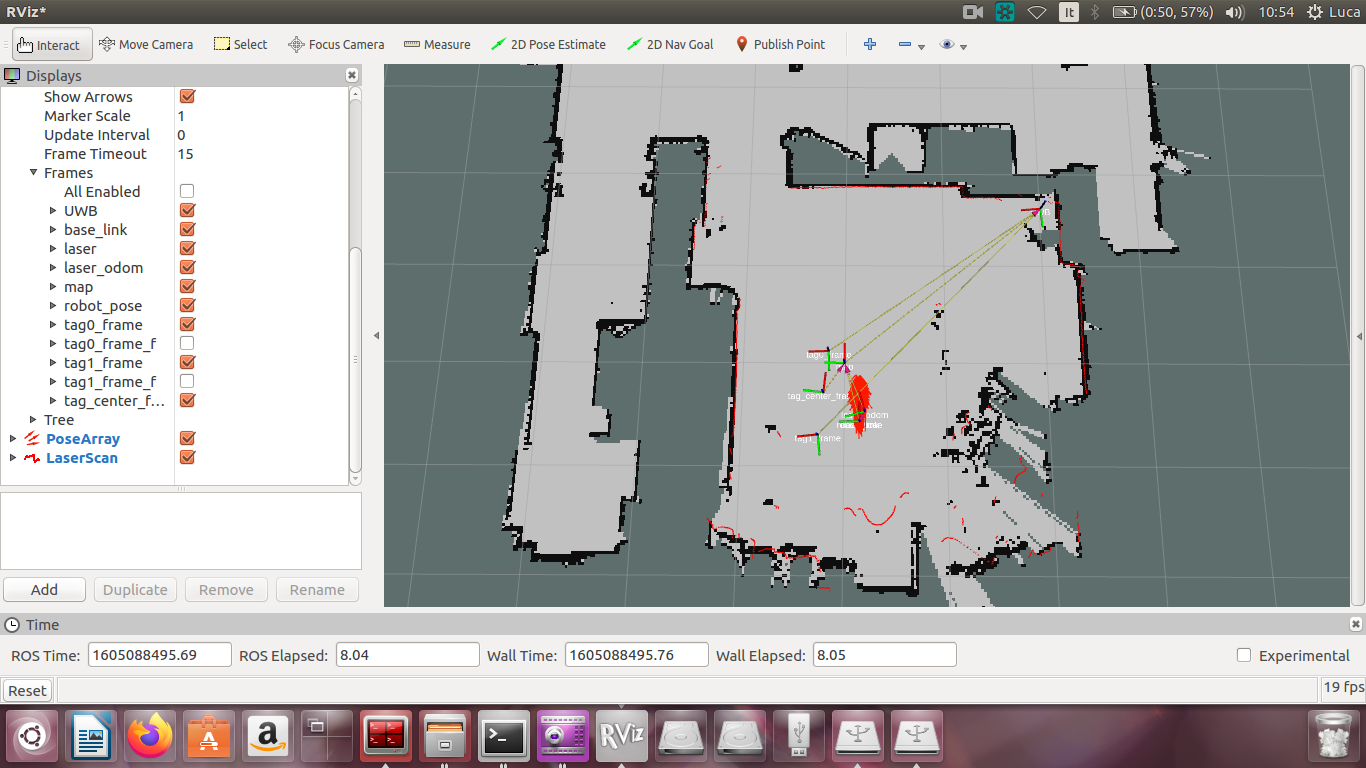
\includegraphics[width=.6\linewidth]{Capitolo3/Figs/esperimento2_1_situazione_di_partenza.png} }
% 
%\subfloat[Pose fix forzato errato]{
%	\label{subfig:esp1_2}
%     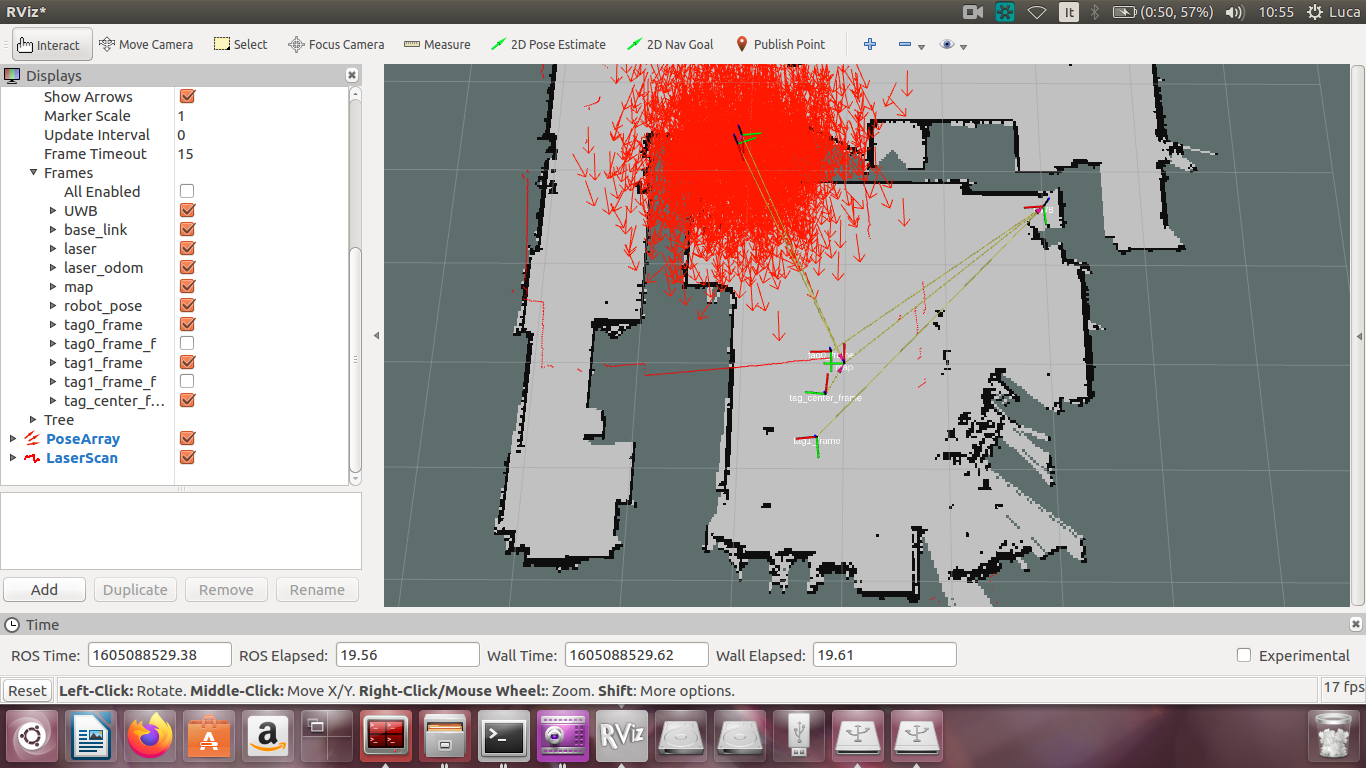
\includegraphics[width=.6\linewidth]{Capitolo3/Figs/esperimento2_2_pose_fix_forzato_errato.png} } 
%\end{figure}
%\begin{figure}[ht]\ContinuedFloat
%\subfloat[Pose fix autocorrezione]{
%	\label{subfig:esp1_3}
%     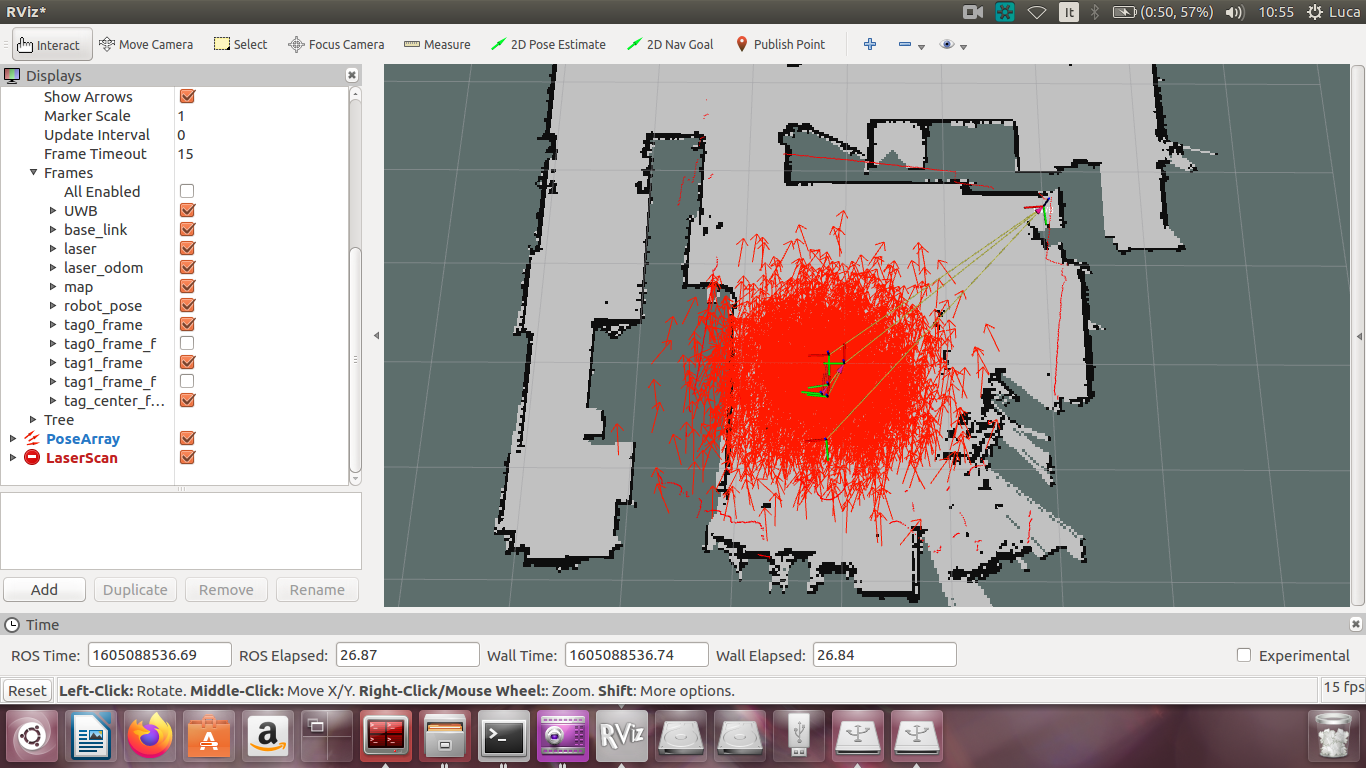
\includegraphics[width=.6\linewidth]{Capitolo3/Figs/esperimento2_3_pose_fix_automatico_di_correzione.png} } 
 
%\subfloat[Risultato finale]{
%	\label{subfig:esp1_4}
 %   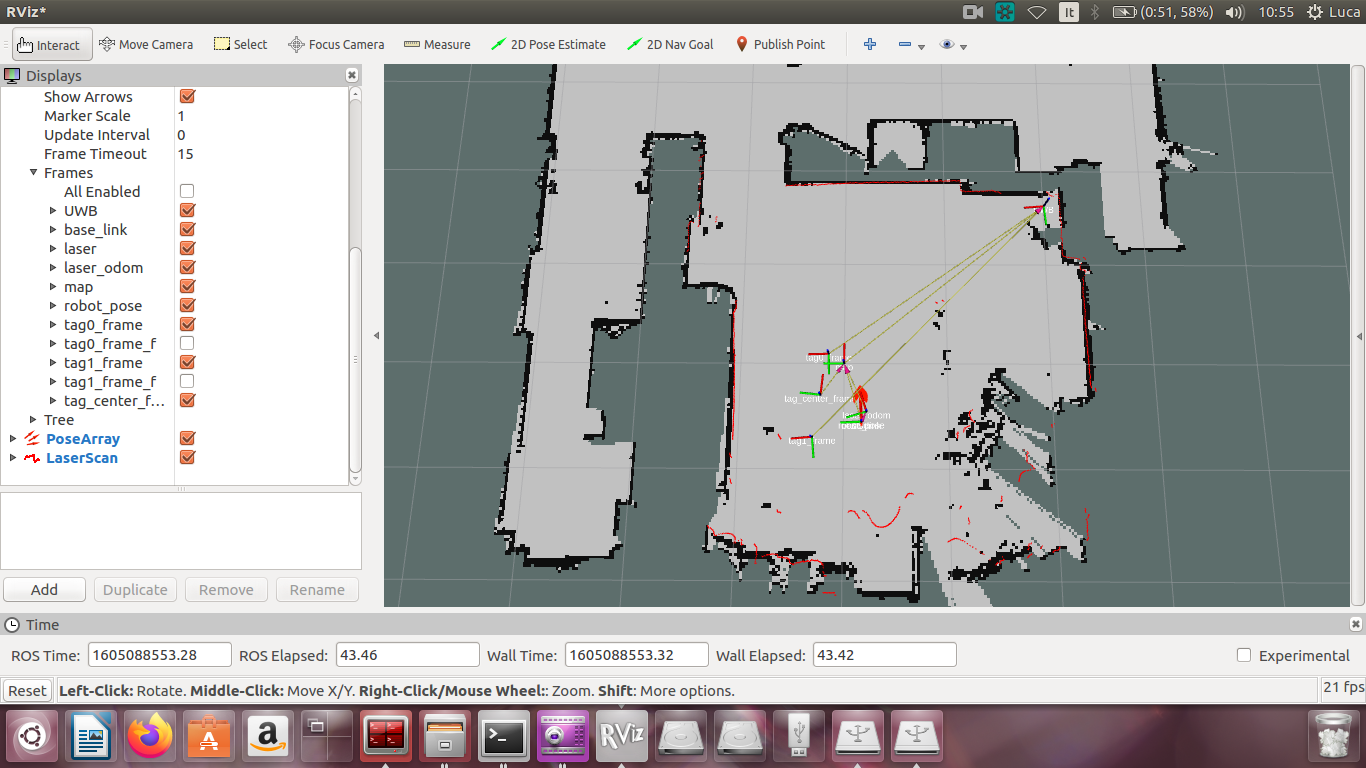
\includegraphics[width=.6\linewidth]{Capitolo3/Figs/esperimento2_4_risultato_finale.png}} 
%     
%\caption{Esperimento 1}
%\label{fig:esperimento_1}
% 
%\end{figure}
\begin{figure}[h]
\begin{subfigure}{.5\textwidth}
  \centering
  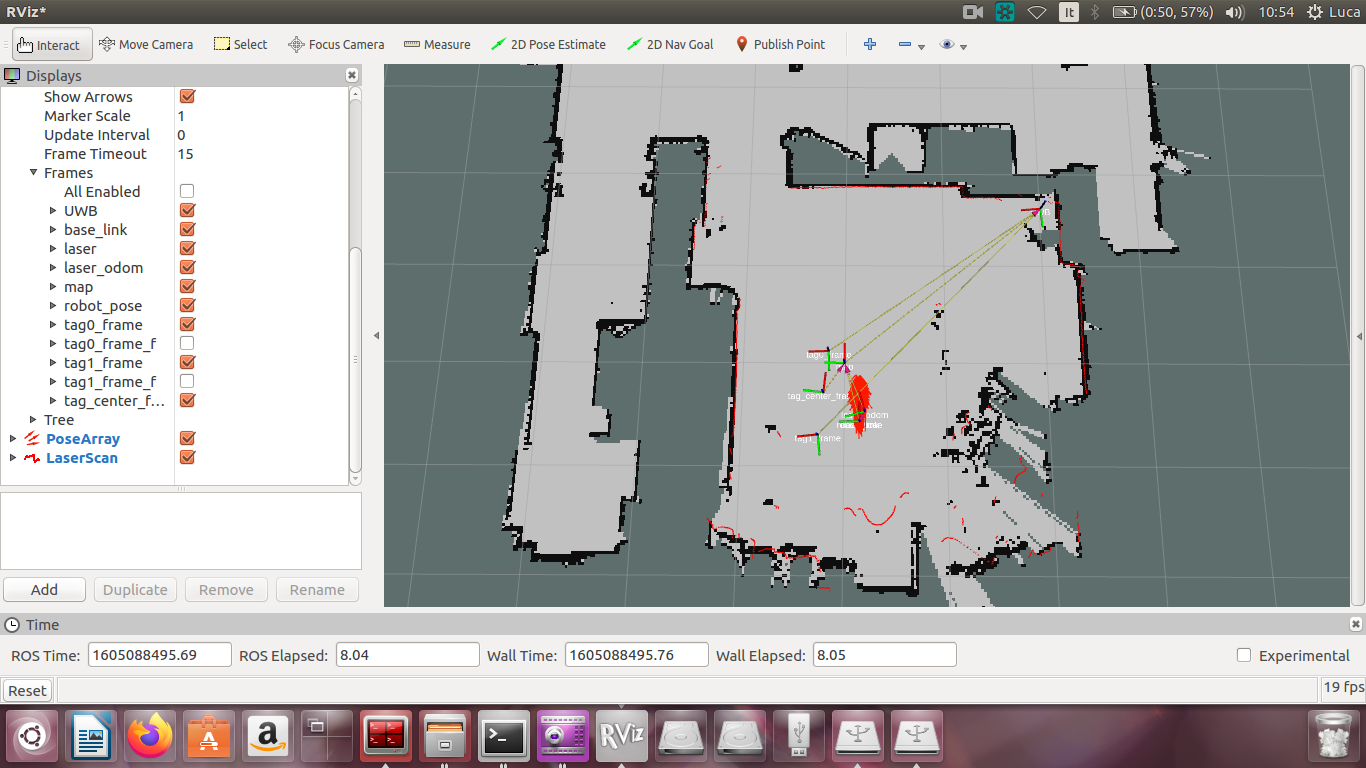
\includegraphics[width=1\linewidth]{Capitolo3/Figs/esperimento2_1_situazione_di_partenza.png}  
  \caption{Situazione di partenza}
	\label{subfig:esp1_1}
\end{subfigure}
\begin{subfigure}{.5\textwidth}
  \centering
  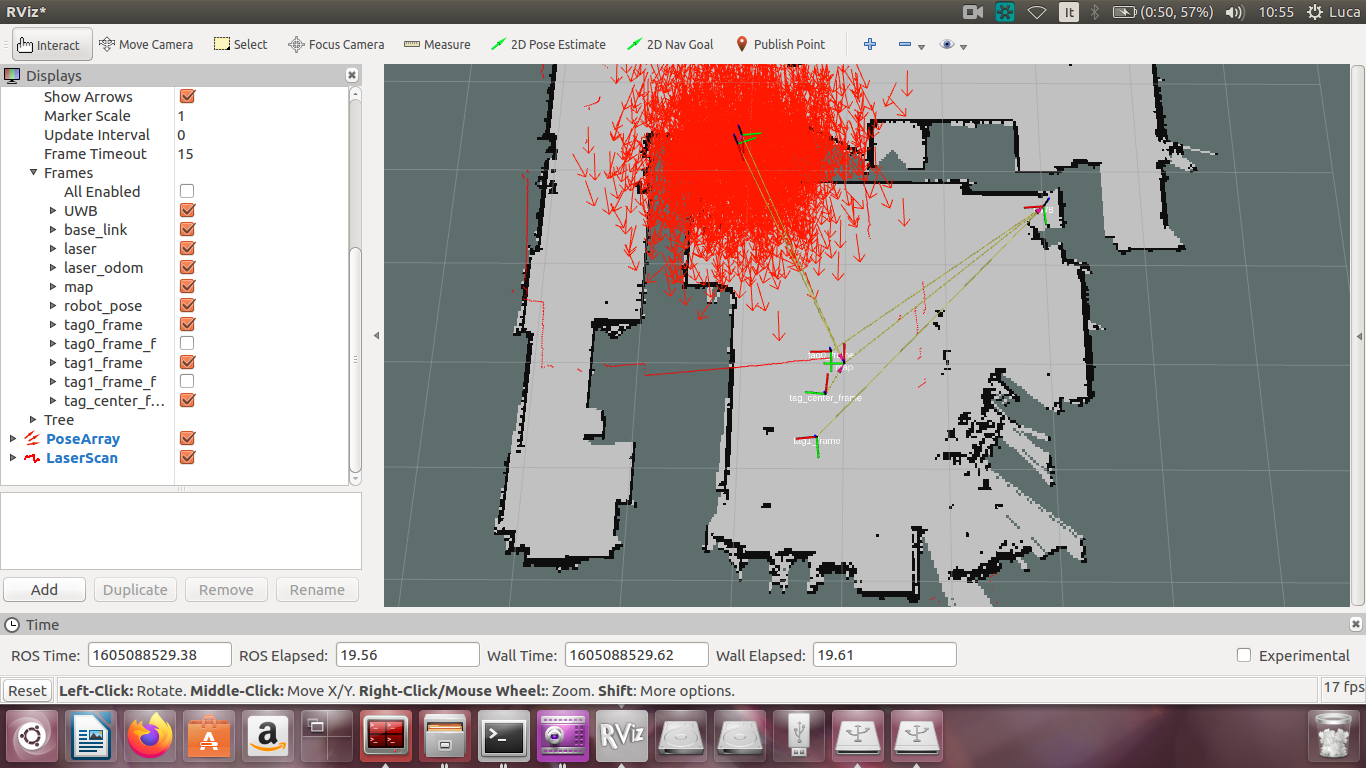
\includegraphics[width=1\linewidth]{Capitolo3/Figs/esperimento2_2_pose_fix_forzato_errato.png}  
  \caption{Pose fix forzato errato}
	\label{subfig:esp1_2}
\end{subfigure}
\end{figure}
\clearpage

\begin{figure}[ht]\ContinuedFloat
\begin{subfigure}{.5\textwidth}
  \centering
  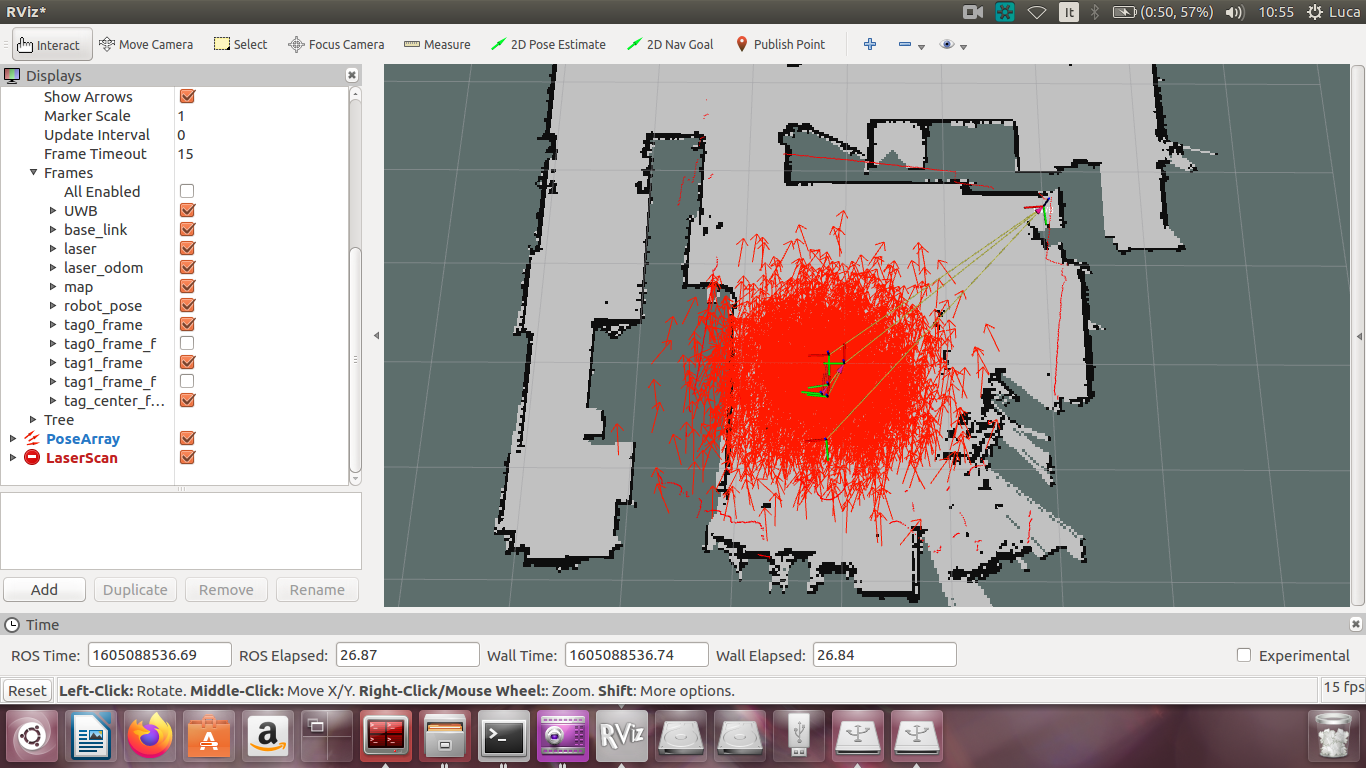
\includegraphics[width=1\linewidth]{Capitolo3/Figs/esperimento2_3_pose_fix_automatico_di_correzione.png}  
  \caption{Pose fix autocorrezione}
	\label{subfig:esp1_3}
\end{subfigure}
\begin{subfigure}{.5\textwidth}
  \centering
  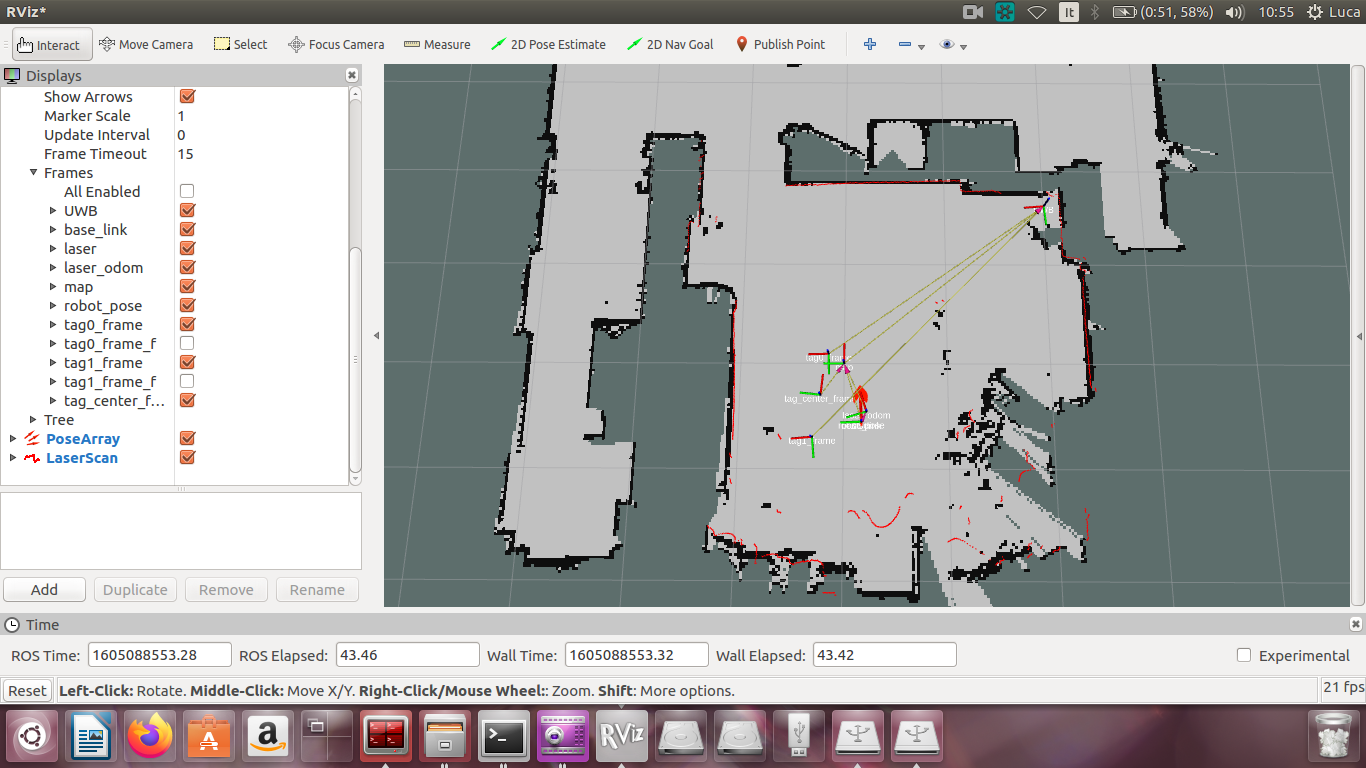
\includegraphics[width=1\linewidth]{Capitolo3/Figs/esperimento2_4_risultato_finale.png}  
  \caption{Risultato finale}
  	\label{subfig:esp1_4}
\end{subfigure}
\caption{Esperimento 1}
\end{figure}

\bigskip
\bigskip
\bigskip
\bigskip

% ********************************** Sezione 3.2  **************************************
\section{Esperimento 2 - Fix di posa durante navigazione in più stanze}
Nel secondo esperimento ci si è posti nelle condizioni di funzionamento standard, con il robot che naviga tra più stanze, per verificare come si comporta l'algoritmo di localizzazione con i relativi meccanismi di correzione.


La procedura funziona bene e senza problemi finché il robot si trova nella stanza in cui sono presenti le ancore UWB, il veicolo naviga senza problemi e la localizzazione, che avviene tramite AMCL, è sempre molto precisa (Figure~\ref{subfig:esp2_1a},~\ref{subfig:esp2_1b},~\ref{subfig:esp2_2a},~\ref{subfig:esp2_2b}).  

Ciò non succede quando tale stanza viene lasciata, infatti spostandosi in altri ambienti le tag UWB risentono di forti disturbi e questo si traduce in una discordanza tra la posa stimata da AMCL e quella stimata dalle tag, che iniziano ad inviare continui fix di posizione errati (Figure~\ref{subfig:esp2_3a},~\ref{subfig:esp2_3b}).

Questo porta l'algoritmo AMCL a reinizializzarsi di continuo in punti sempre diversi e quasi mai corretti, generando un malfunzionamento di tutta la procedura di localizzazione, che in alcuni casi finisce addirittura per fallire completamente.


Riportando il veicolo nella stanza coperta dalle ancore, dove il segnale UWB risulta molto più stabile e corretto, il tutto riprende a funzionare correttamente (Figure~\ref{subfig:esp2_4a},~\ref{subfig:esp2_4b}).
\label{section3.2}
\clearpage
\begin{figure}
\begin{subfigure}{.5\textwidth}
  \centering
  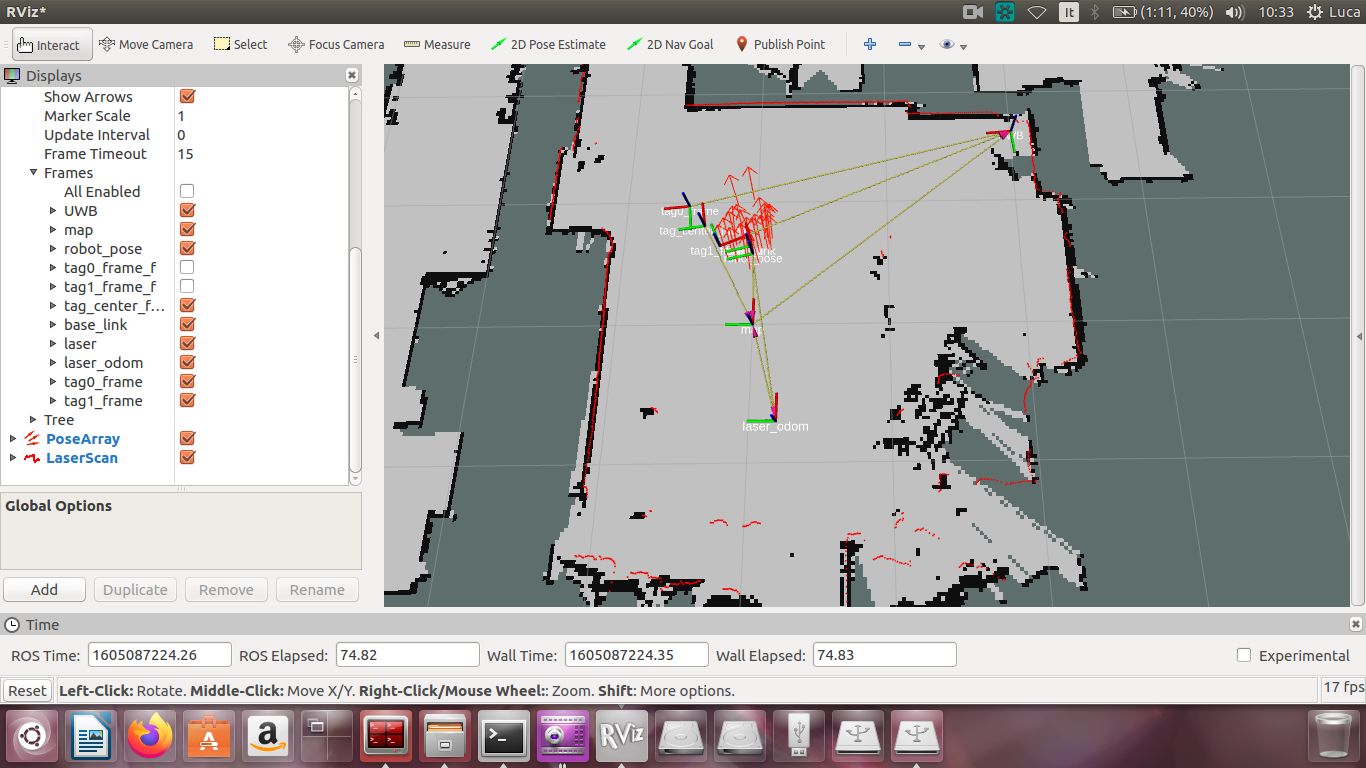
\includegraphics[width=1\linewidth]{Capitolo3/Figs/esperimento1_1a.png}  
  \caption{Punto di partenza - \texttt{Rviz}}
  \label{subfig:esp2_1a}
\end{subfigure}
\begin{subfigure}{.5\textwidth}
  \centering
  \includegraphics[width=1\linewidth]{Capitolo3/Figs/esperimento1_1b.png}  
  \caption{Punto di partenza}
  \label{subfig:esp2_1b}
\end{subfigure}

\vskip\baselineskip

\begin{subfigure}{.5\textwidth}
  \centering
  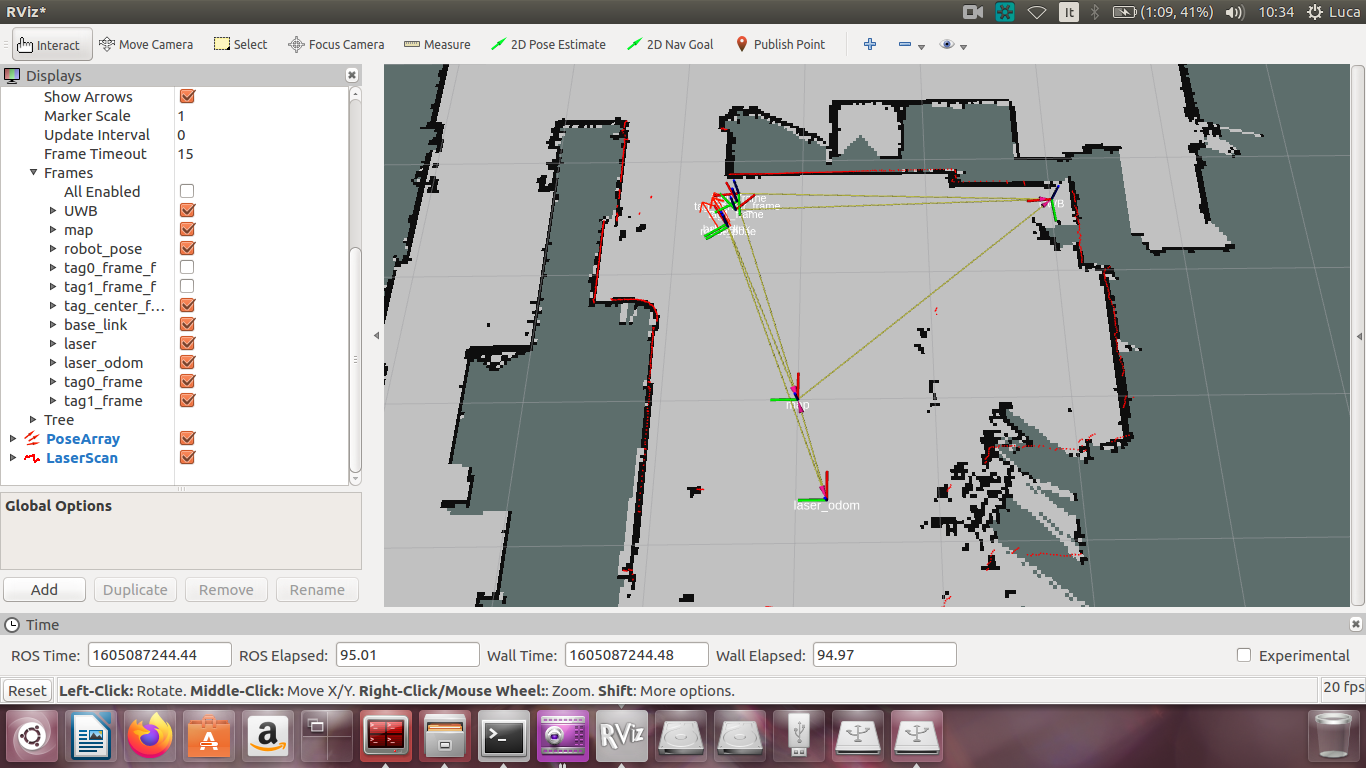
\includegraphics[width=1\linewidth]{Capitolo3/Figs/esperimento1_2a.png}  
  \caption{Prosegue dritto verso la porta - \texttt{Rviz}}
  \label{subfig:esp2_2a}
\end{subfigure}
\begin{subfigure}{.5\textwidth}
  \centering
  \includegraphics[width=1\linewidth]{Capitolo3/Figs/esperimento1_2b.png}  
  \caption{Prosegue dritto verso la porta}
  \label{subfig:esp2_2b}
\end{subfigure}

\vskip\baselineskip

\begin{subfigure}{.5\textwidth}
  \centering
  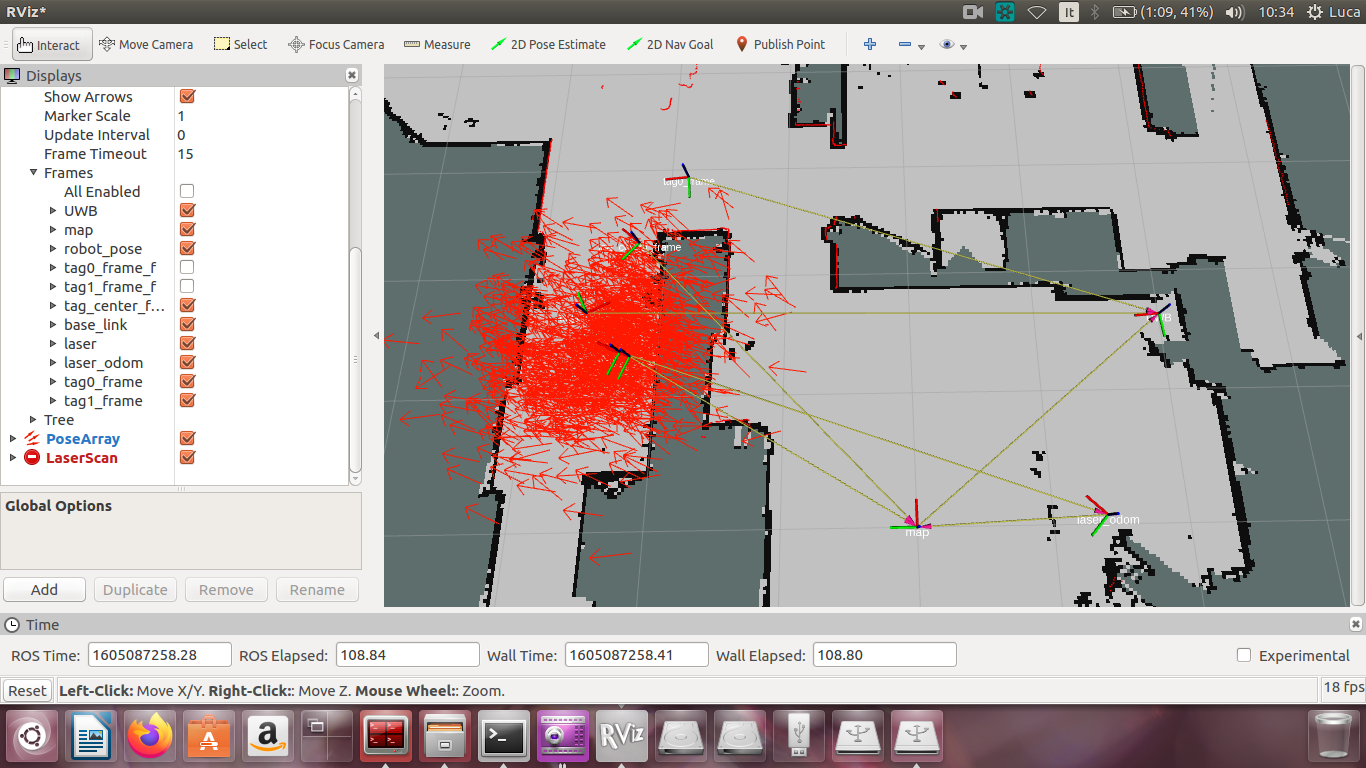
\includegraphics[width=1\linewidth]{Capitolo3/Figs/esperimento1_3a.png}  
  \caption{Fuori dalla stanza - \texttt{Rviz}}
  \label{subfig:esp2_3a}
\end{subfigure}
\begin{subfigure}{.5\textwidth}
  \centering
  \includegraphics[width=1\linewidth]{Capitolo3/Figs/esperimento1_3b.png}  
  \caption{Fuori dalla stanza}
  \label{subfig:esp2_3b}
\end{subfigure}

\vskip\baselineskip

\begin{subfigure}{.5\textwidth}
  \centering
  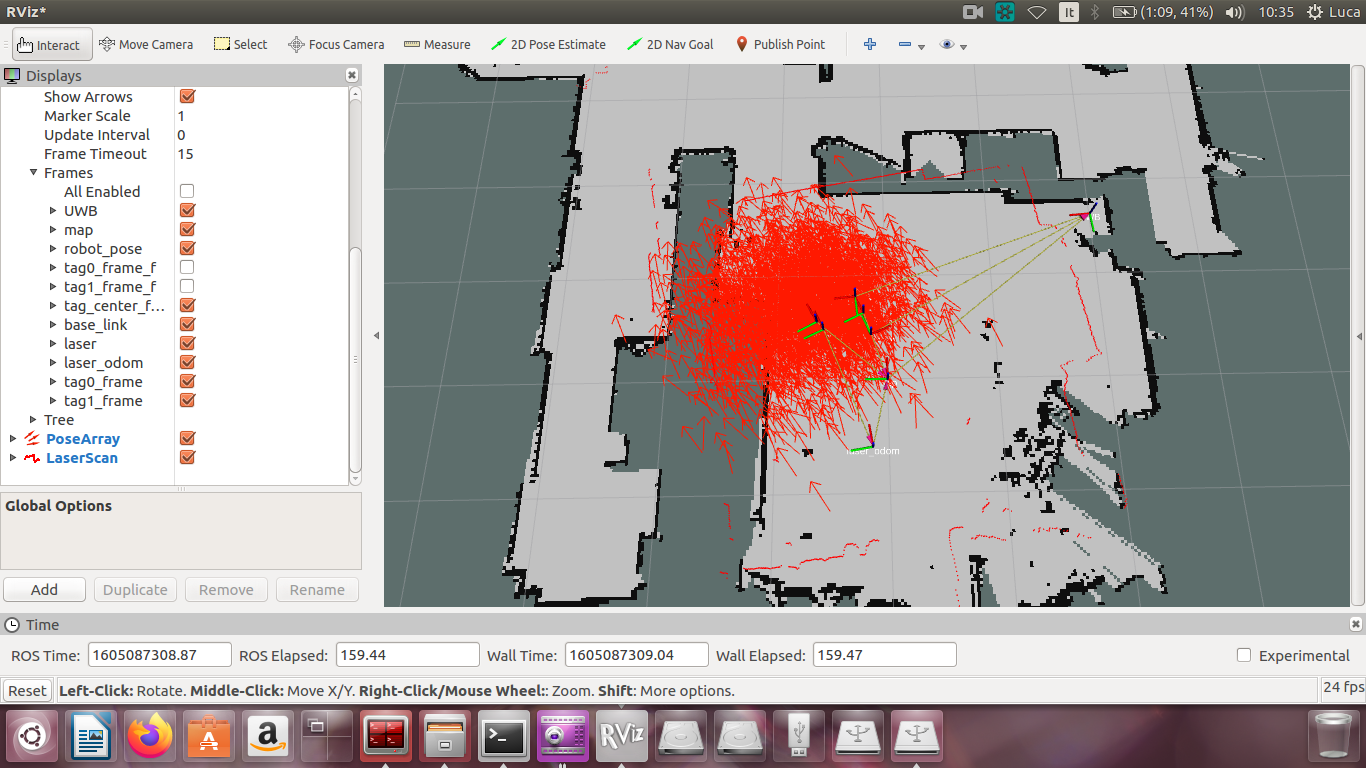
\includegraphics[width=1\linewidth]{Capitolo3/Figs/esperimento1_4a.png}  
  \caption{Ritorno al punto di partenza - \texttt{Rviz}}
  \label{subfig:esp2_4a}
\end{subfigure}
\begin{subfigure}{.5\textwidth}
  \centering
  \includegraphics[width=1\linewidth]{Capitolo3/Figs/esperimento1_4b.png}  
  \caption{Ritorno al punto di partenza}
  \label{subfig:esp2_4b}
\end{subfigure}

\caption[Esperimento 2]{Esperimento 2}
\label{fig:esperimento_2}
\end{figure}
\clearpage
% ********************************** Sezione 3.3 **************************************
\section{Esperimento 3 - Rapimento del robot}
\label{section3.3}
Nel terzo esperimento si è simulata l'eventualità in cui il Lidar potrebbe non riuscire a vedere oppure sia soggetto ad un malfunzionamento. In questo caso l'algoritmo AMCL, non ricevendo scansioni valide, si arresta e smette di inviare le stime di posa del robot. Senza nessun tipo di accorgimento, questo porterebbe la localizzazione ed il relativo controllo a fallire.

Ecco allora subentrare la navigazione puramente basata sul segnale UWB, che, seppur rumoroso e soggetto ad errori, continua a dare una stima della posizione del robot, che si sostituisce temporaneamente a quella che dovrebbe arrivare dal Lidar, permettendo di continuare l'esecuzione del task assegnato.

Nel caso in cui il Lidar torni in linea, tutta la procedura di localizzazione passa di nuovo al funzionamento standard, ovvero Lidar come sensore principale e tag sfruttate solo per correzioni di posa in caso di errori.

Per eseguire questo test si è coperto il sensore Lidar, in modo che le scansioni inviate risultassero nulle e poi si è spostato il robot manualmente in una posizione differente (Figure~\ref{subfig:esp3_2a},~\ref{subfig:esp3_2b},~\ref{subfig:esp3_3a},~\ref{subfig:esp3_3b}). Così facendo, AMCL oltre a non essere in grado di accorgersi delle variazioni, smette di inviare pose aggiornate. 

Durante lo spostamento, come anticipato, sono le UWB a mandare il messaggio con la posa del robot aggiornata (Figura~\ref{subfig:esp3_4b}).

Una volta posizionato in un nuovo punto, differente da quello di partenza, il Lidar è stato nuovamente scoperto. Con il ritorno dei messaggi sul topic \texttt{/scan}, è arrivato anche il fix di posa per reinizializzare il filtro a particelle, che come si può apprezzare nelle (Figure~\ref{subfig:esp3_5a},~\ref{subfig:esp3_5b},~\ref{subfig:esp3_6a},~\ref{subfig:esp3_7a},~\ref{subfig:esp3_7b}) converge.

A questo punto la navigazione può continuare normalmente.

\clearpage
\begin{figure}[h]
\begin{minipage}[c]{\textwidth}
  \centering
\begin{subfigure}{.5\textwidth}
  %\centering
  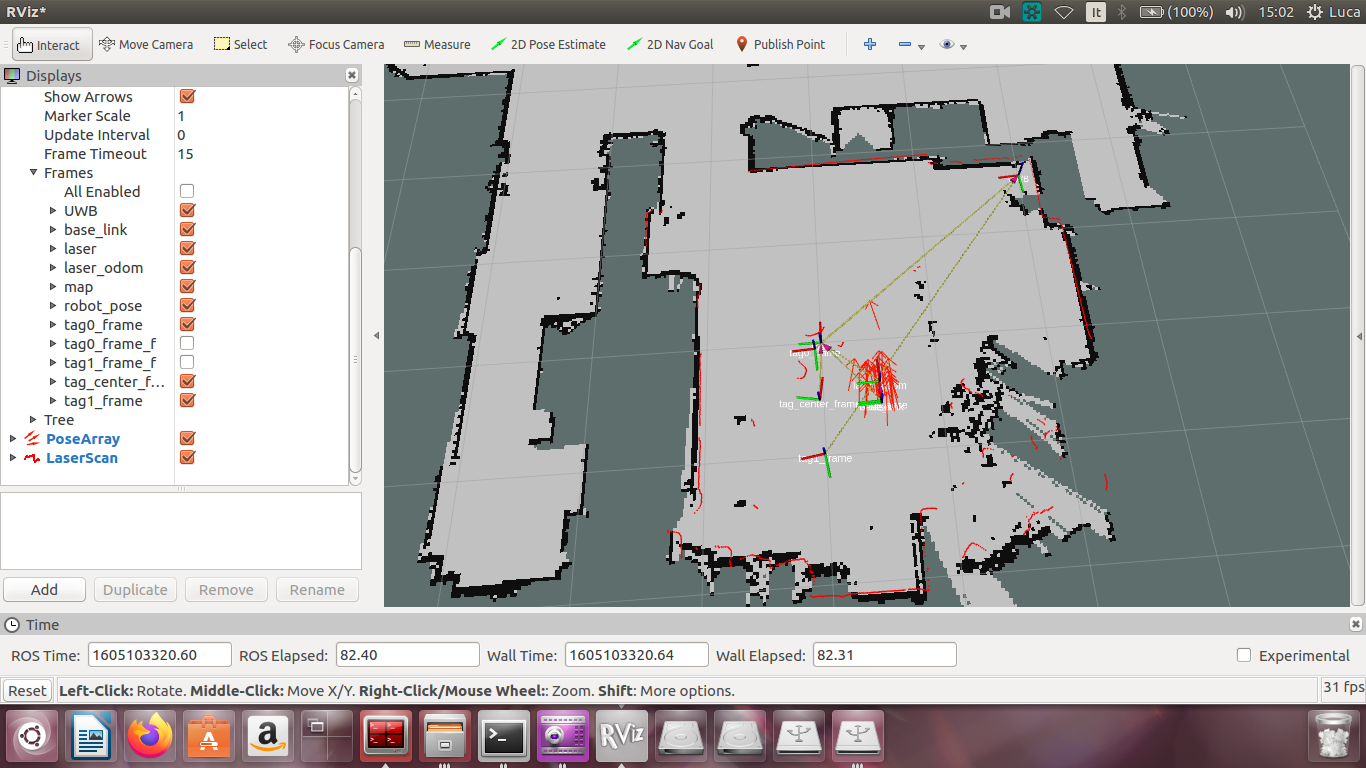
\includegraphics[width=1\linewidth]{Capitolo3/Figs/esperimento3_1a.png}  
  \caption{Punto di partenza - \texttt{Rviz}}
  \label{subfig:esp3_1a}
\end{subfigure}
\end{minipage}

\vskip\baselineskip

\begin{subfigure}{.5\textwidth}
  \centering
  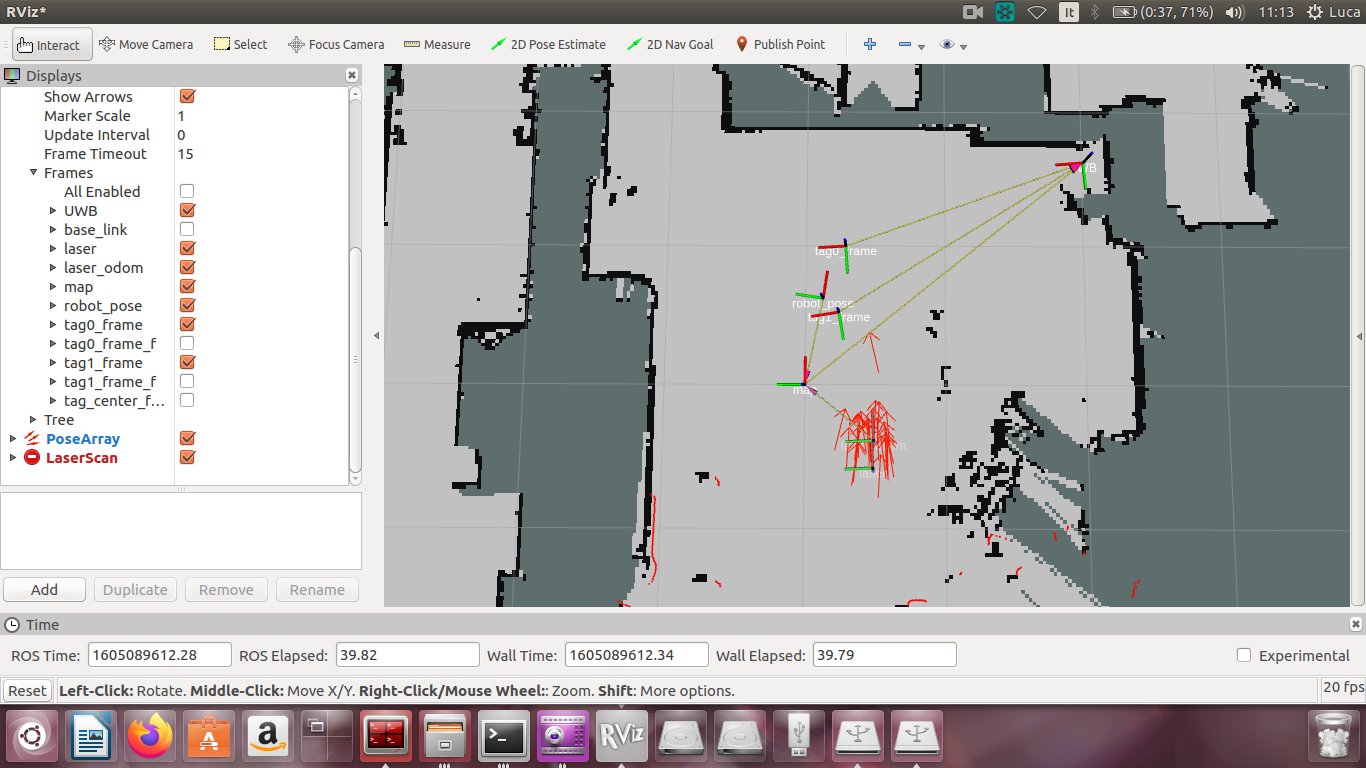
\includegraphics[width=1\linewidth]{Capitolo3/Figs/esperimento3_2a_rapimento.png}  
  \caption{Rapimento - \texttt{Rviz}}
  \label{subfig:esp3_2a}
\end{subfigure}
\begin{subfigure}{.5\textwidth}
  \centering
  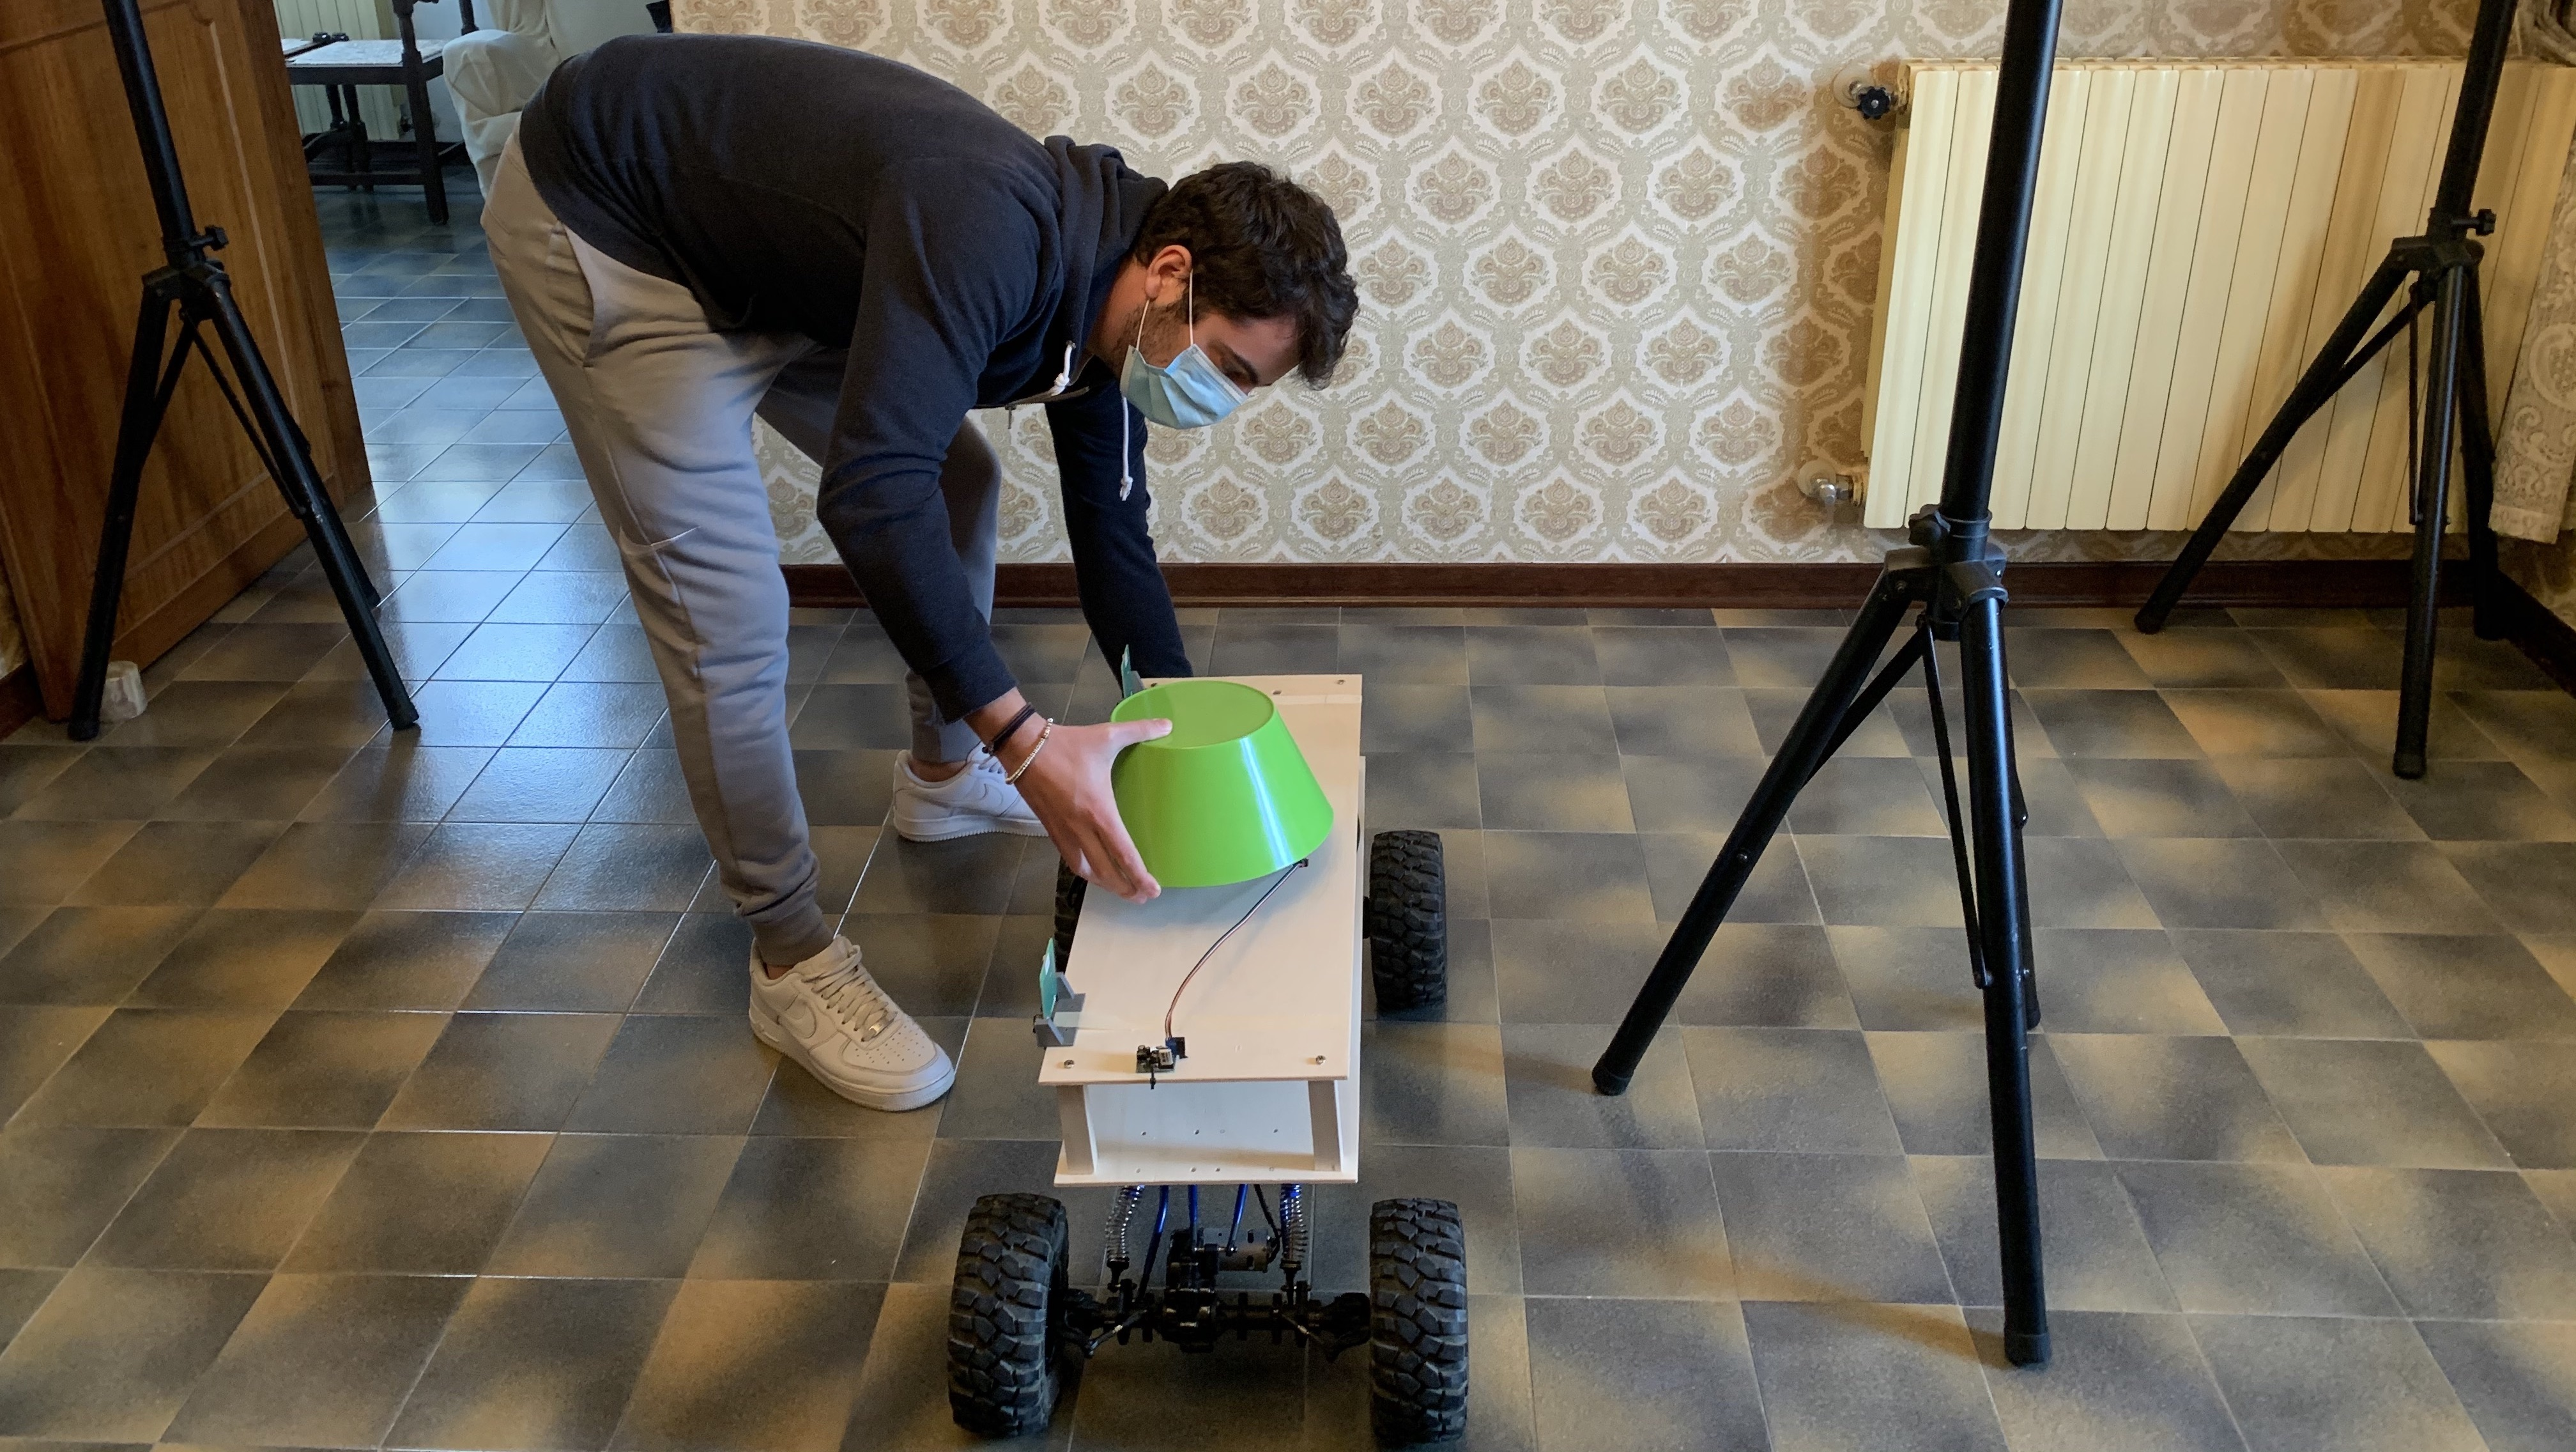
\includegraphics[width=1\linewidth]{Capitolo3/Figs/esperimento3_2b.jpg}  
  \caption{Rapimento}
  \label{subfig:esp3_2b}
\end{subfigure}

\vskip\baselineskip

\begin{subfigure}{.5\textwidth}
  \centering
  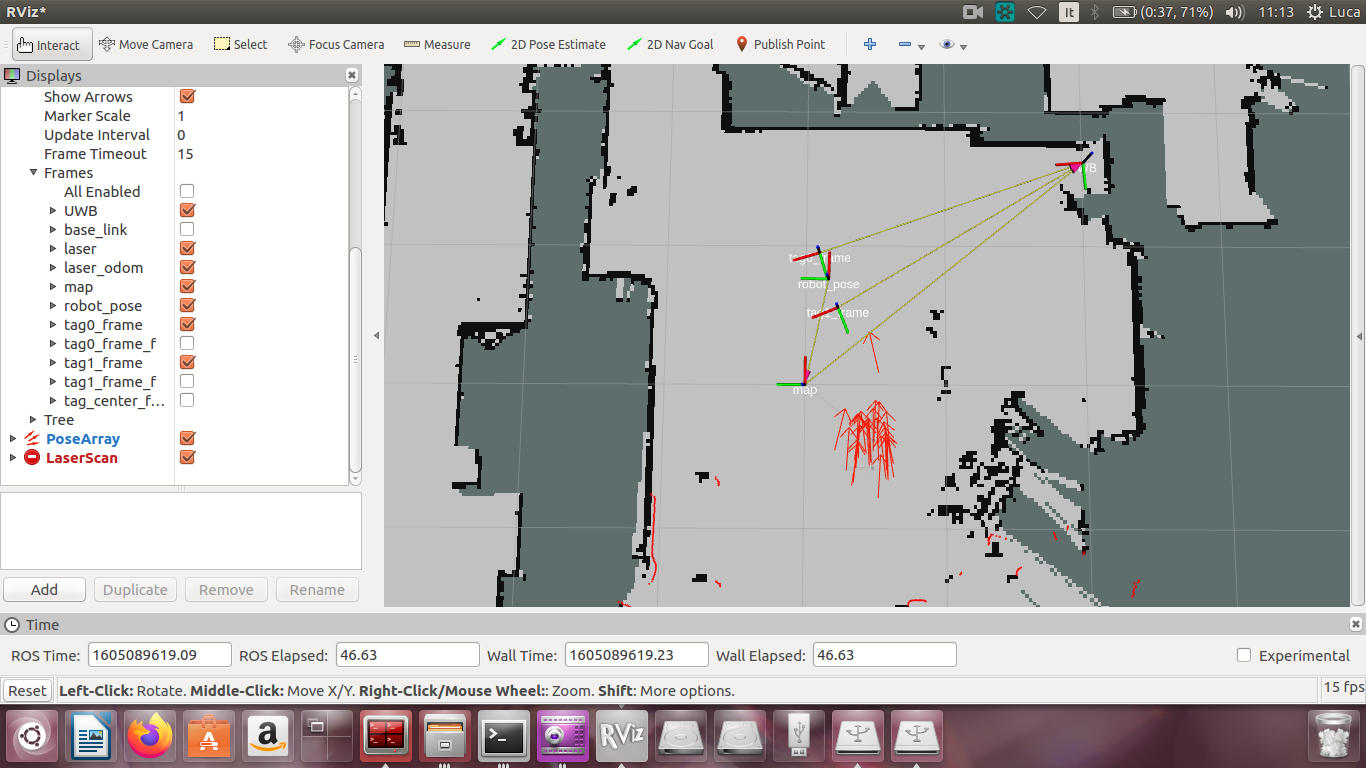
\includegraphics[width=1\linewidth]{Capitolo3/Figs/esperimento3_3a_tag_center_sostituisce_robot_pose_e_si_vedono_i_vecchi_frame.png}  
  \caption{\texttt{tag\_center} sostituisce \texttt{robot\_pose} e si vedono i vecchi frame - \texttt{Rviz}}
  \label{subfig:esp3_3a}
\end{subfigure}
\begin{subfigure}{.5\textwidth}
  \centering
  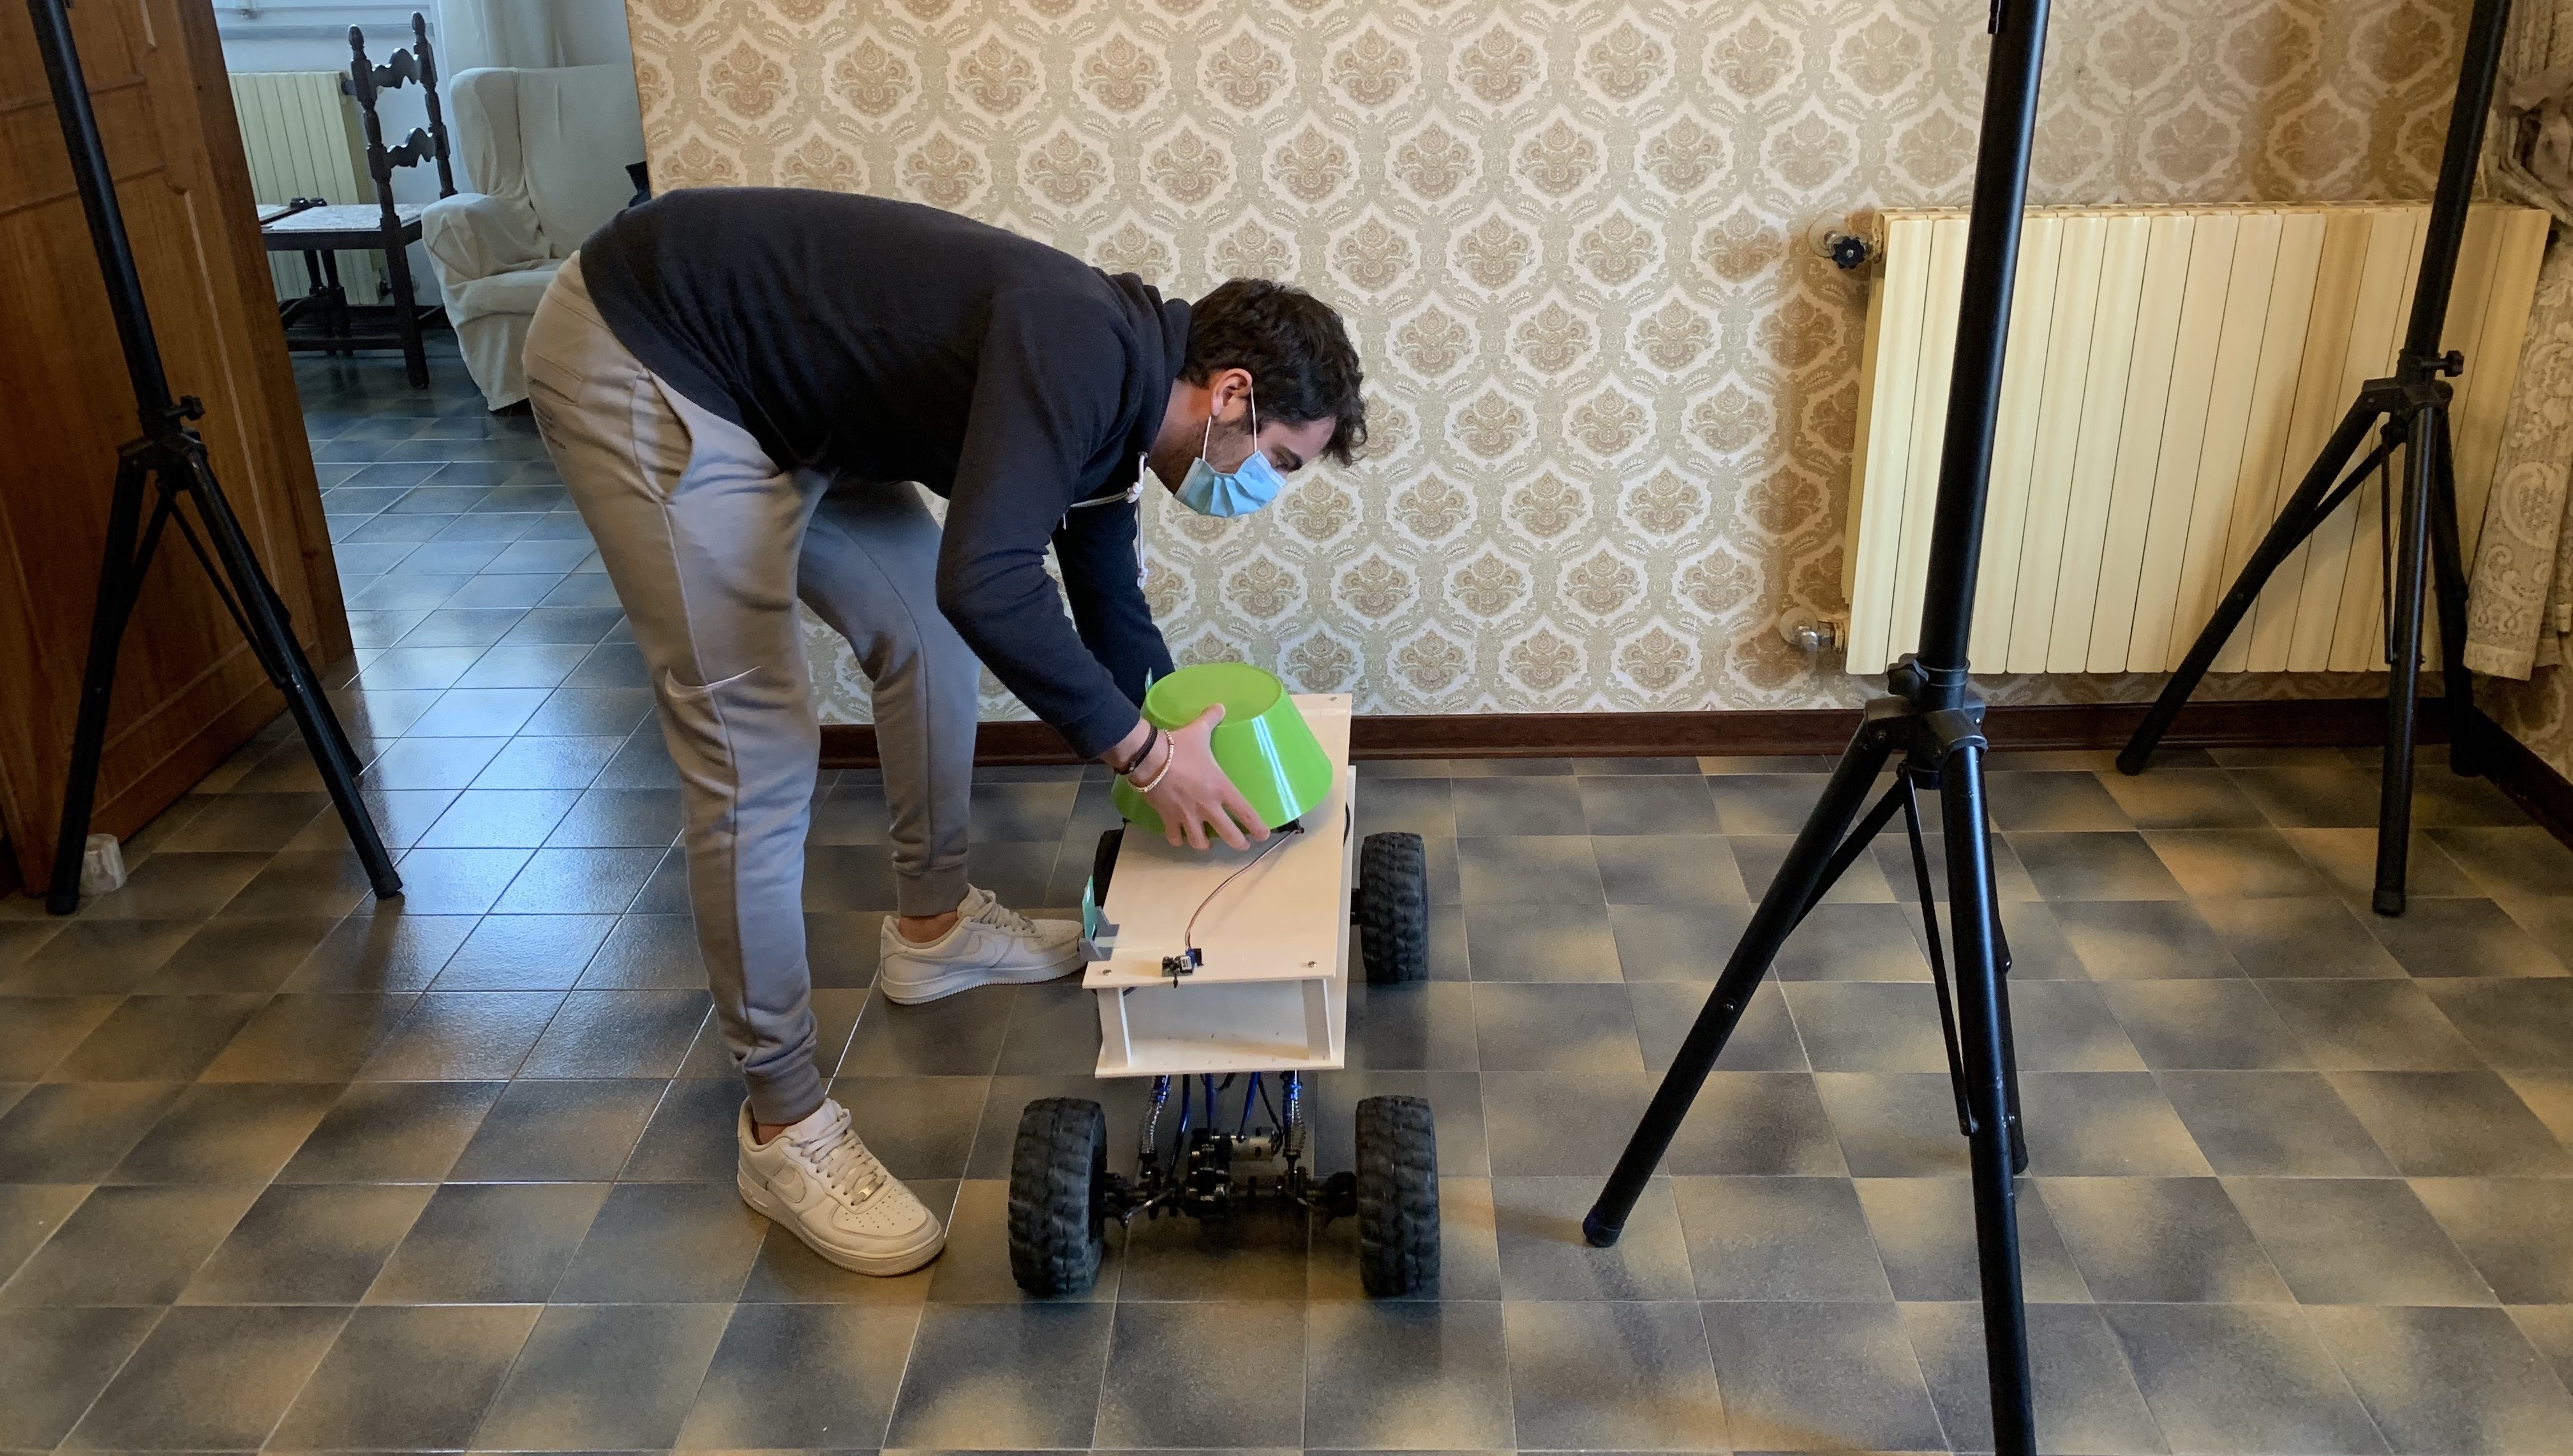
\includegraphics[width=1\linewidth]{Capitolo3/Figs/esperimento3_3b.jpg}  
    \caption{Spostamento mantenendo il sensore Lidar coperto}
  \label{subfig:esp3_3b}
\end{subfigure}

\vskip\baselineskip

\begin{minipage}[c]{\textwidth}
  \centering
\begin{subfigure}{.5\textwidth}
  \centering
  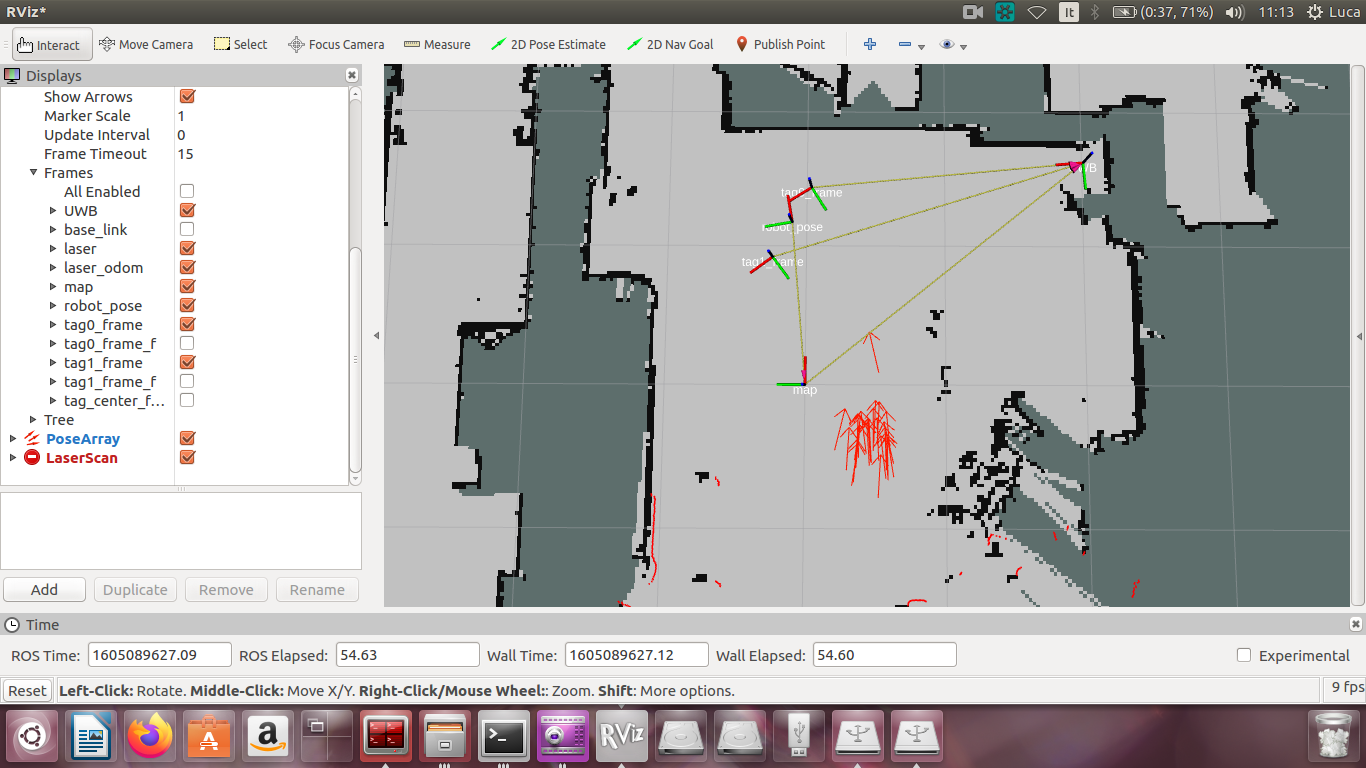
\includegraphics[width=1\linewidth]{Capitolo3/Figs/esperimento3_4a_tag_center_sostituisce_robot_pose.png}  
  \caption{\texttt{tag\_center} sostituisce \texttt{robot\_pose}}
  \label{subfig:esp3_4b}
\end{subfigure}
\end{minipage}
\end{figure}

\begin{figure}[ht]\ContinuedFloat

\begin{subfigure}{.5\textwidth}
  \centering
  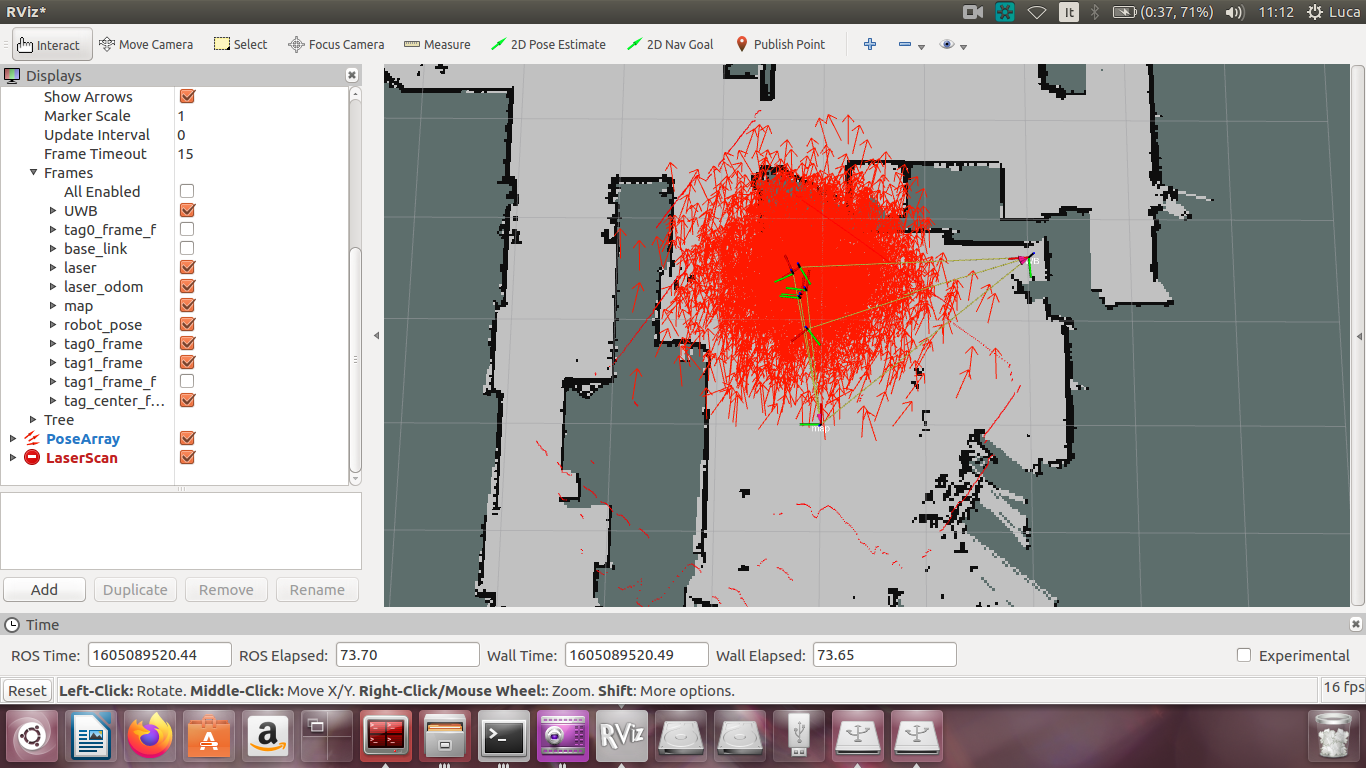
\includegraphics[width=1\linewidth]{Capitolo3/Figs/esperimento3_5a_scopertura_e_fix.png}  
  \caption{Lidar scoperto e fix - \texttt{Rviz}}
  \label{subfig:esp3_5a}
\end{subfigure}
\begin{subfigure}{.5\textwidth}
  \centering
  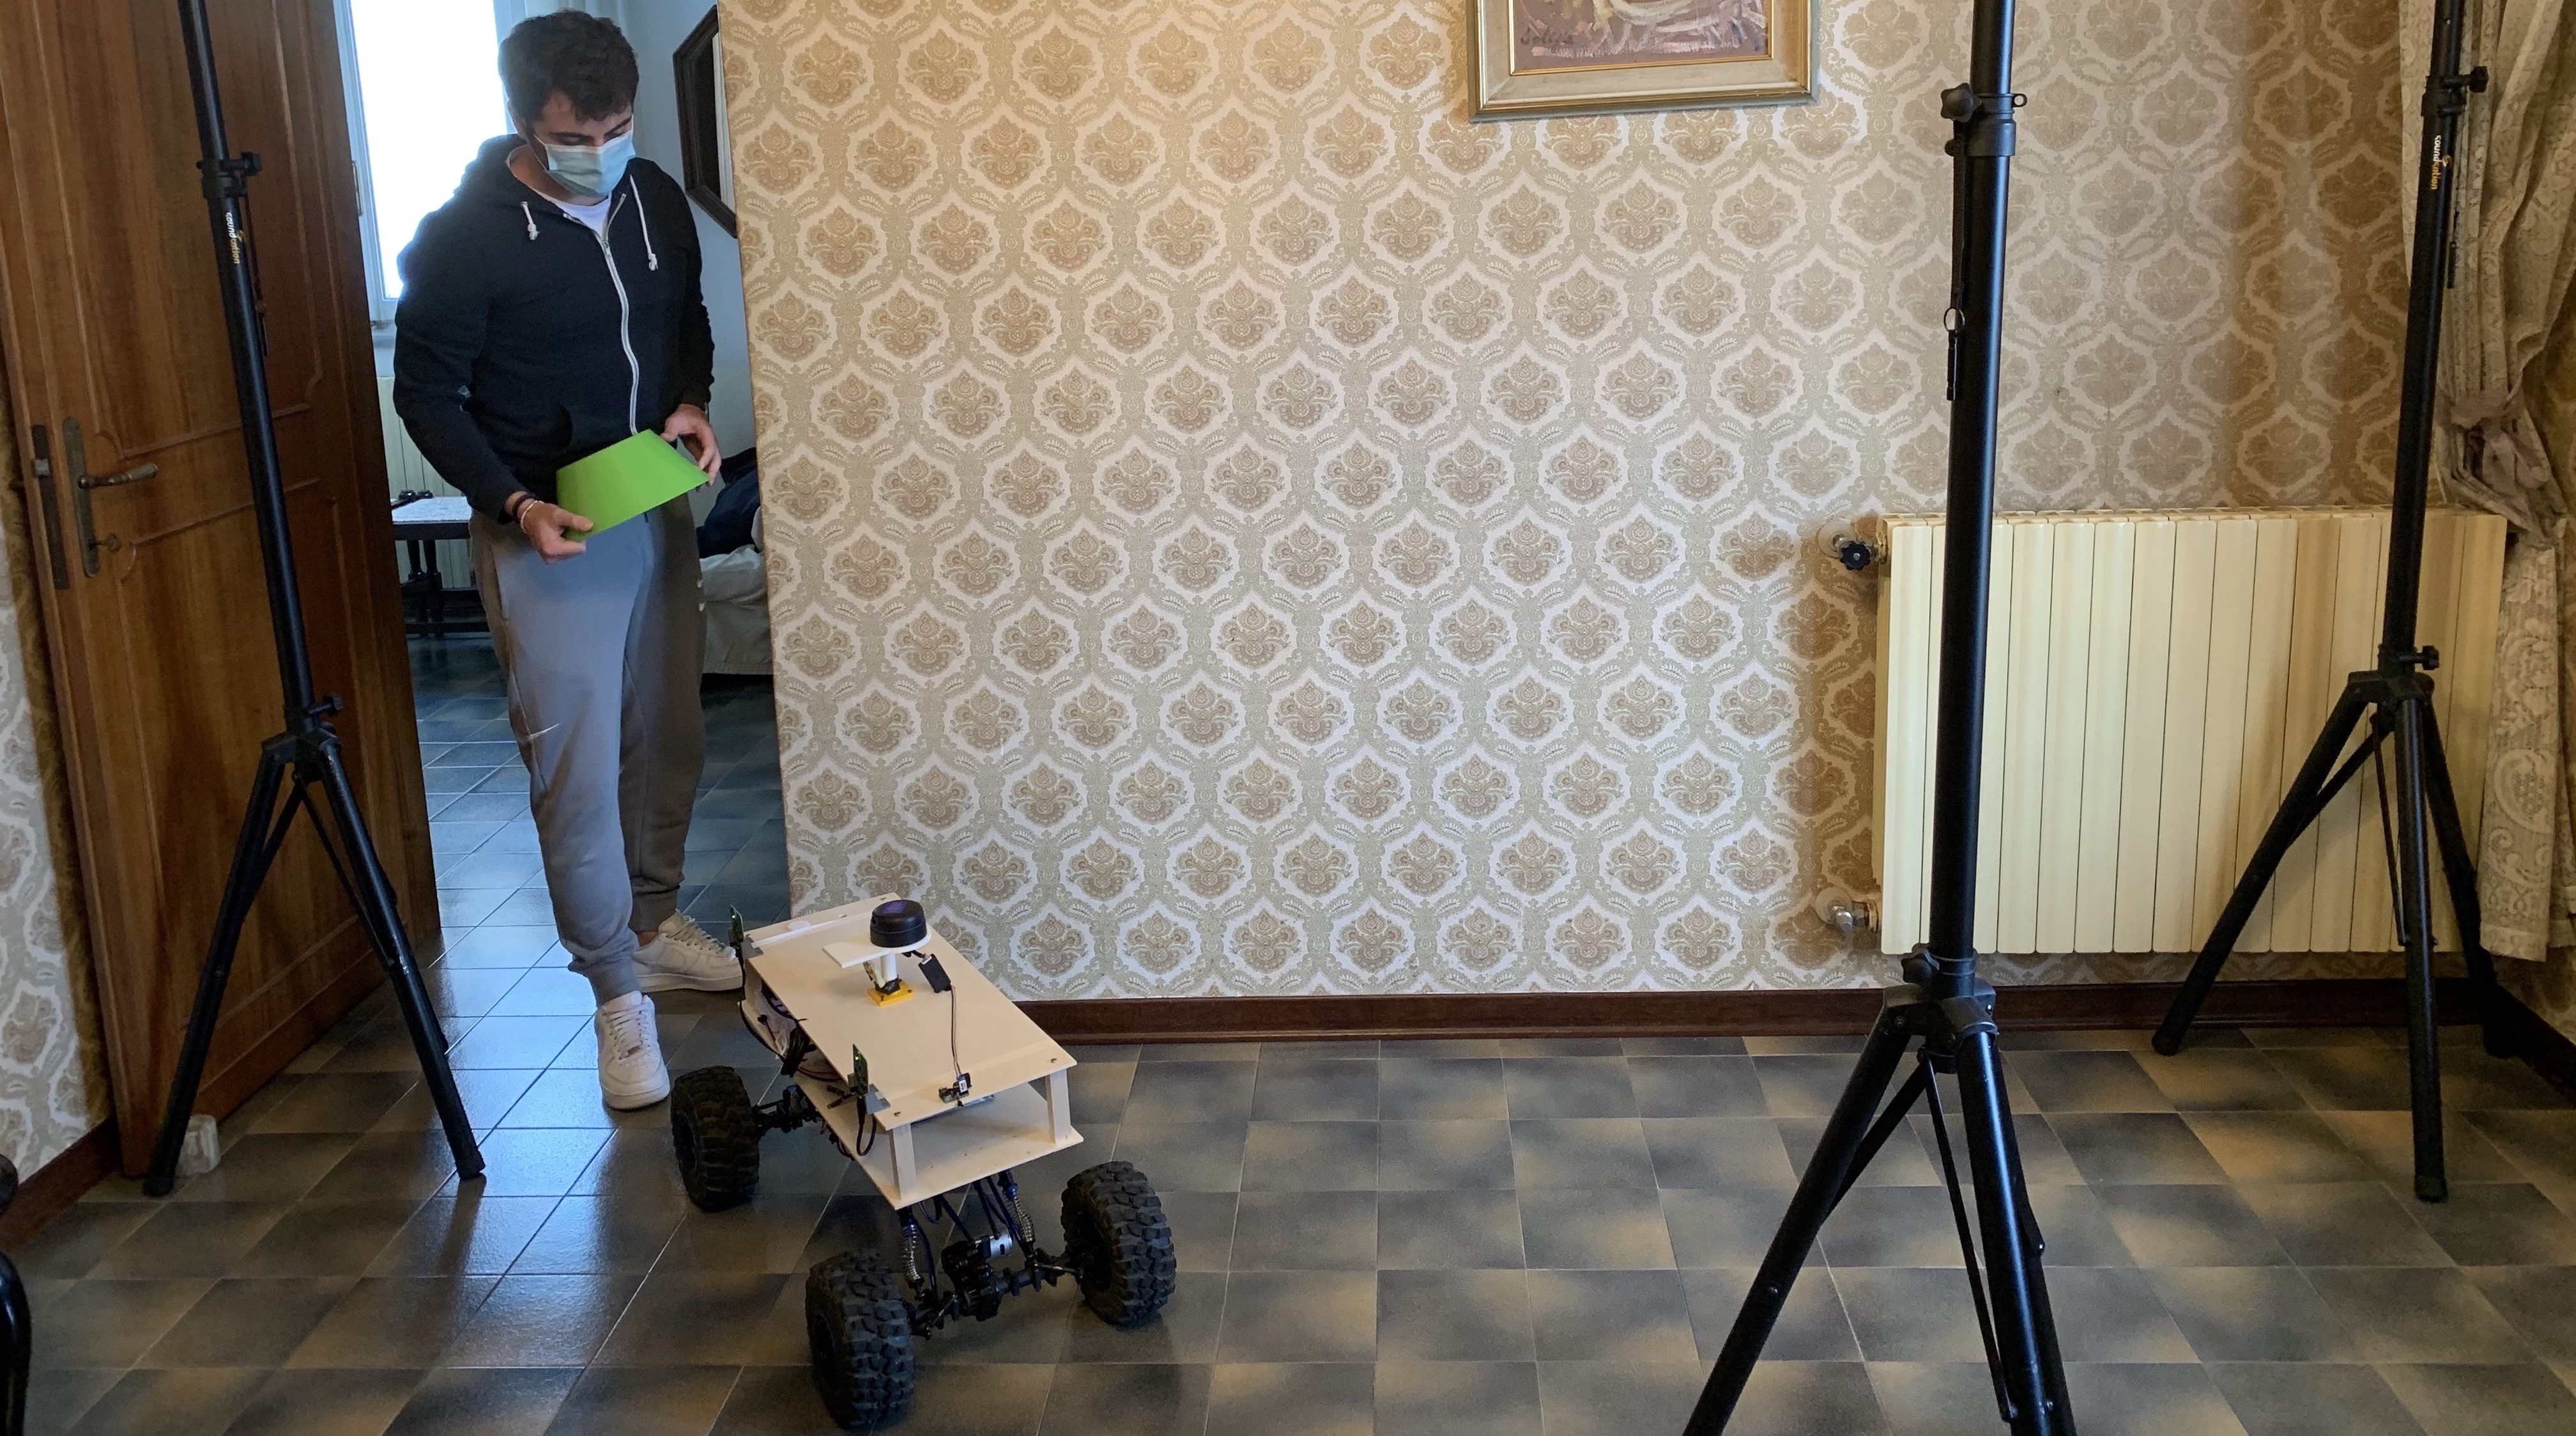
\includegraphics[width=1\linewidth]{Capitolo3/Figs/esperimento3_5b.jpg}  
  \caption{Lidar scoperto e fix}
  \label{subfig:esp3_5b}
\end{subfigure}

\vskip\baselineskip

\begin{minipage}[c]{\textwidth}
  \centering
\begin{subfigure}{.5\textwidth}
  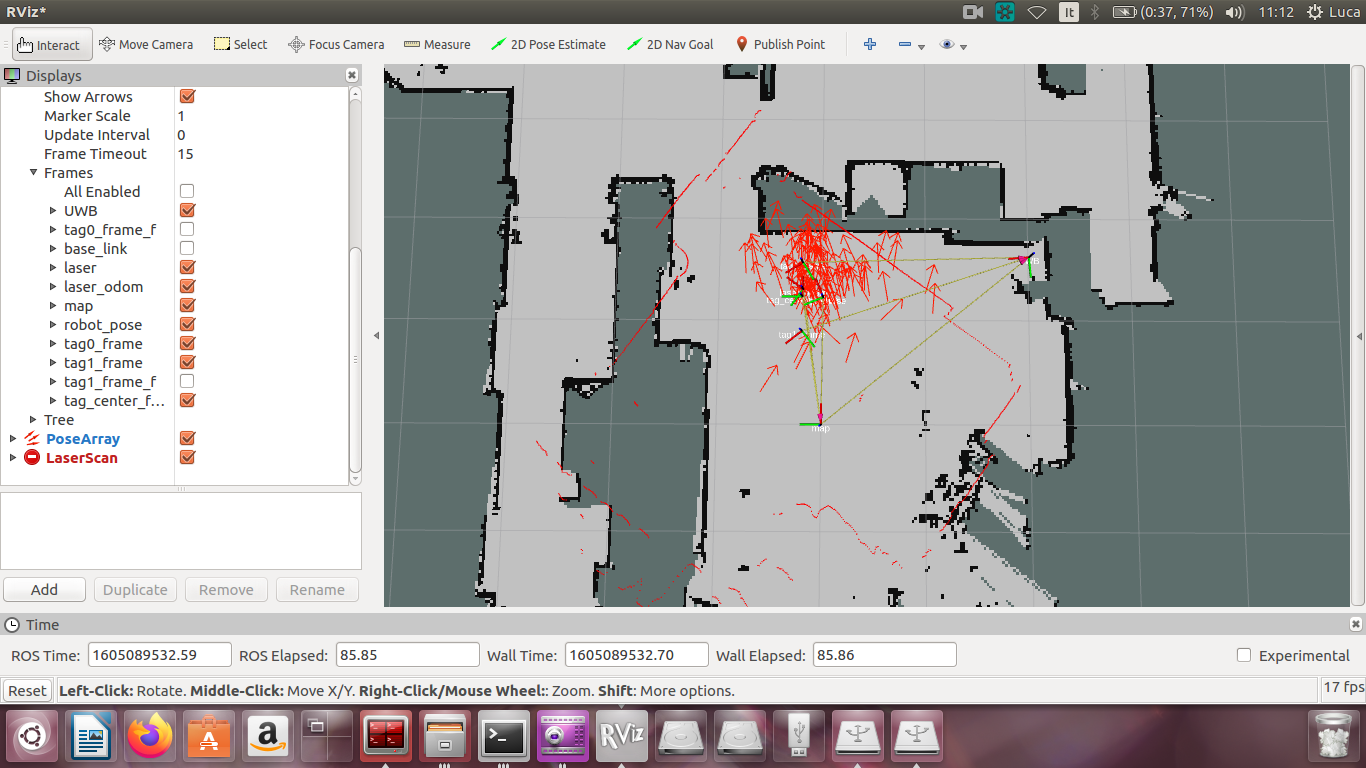
\includegraphics[width=1\linewidth]{Capitolo3/Figs/esperimento3_6a_convergenza.png}  
  \caption{Convergenza ed allineamento in corso - \texttt{Rviz}}
  \label{subfig:esp3_6a}
\end{subfigure}
\end{minipage}

\vskip\baselineskip

\begin{subfigure}{.5\textwidth}
  \centering
  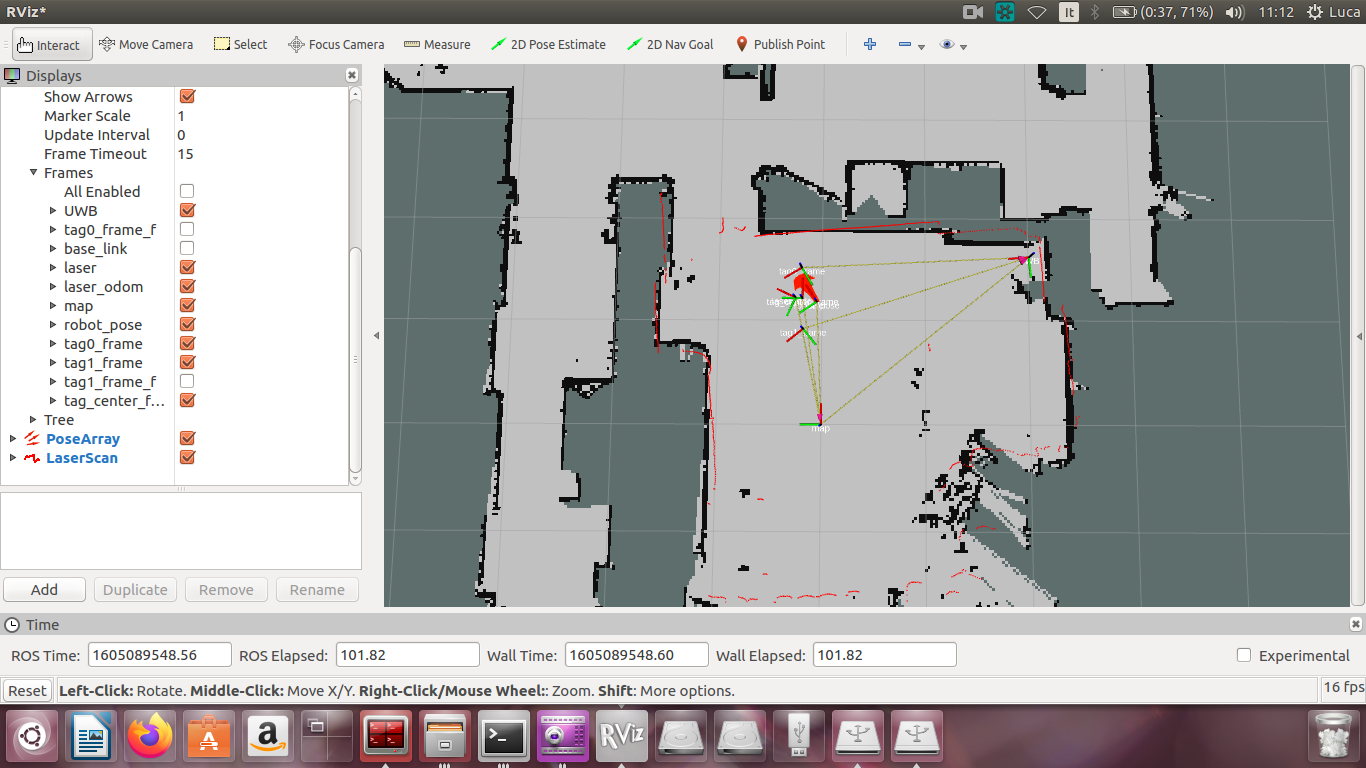
\includegraphics[width=1\linewidth]{Capitolo3/Figs/esperimento3_7a_fine.png}  
  \caption{Nuovamente pronto a navigare - \texttt{Rviz}}
  \label{subfig:esp3_7a}
\end{subfigure}
\begin{subfigure}{.5\textwidth}
  \centering
  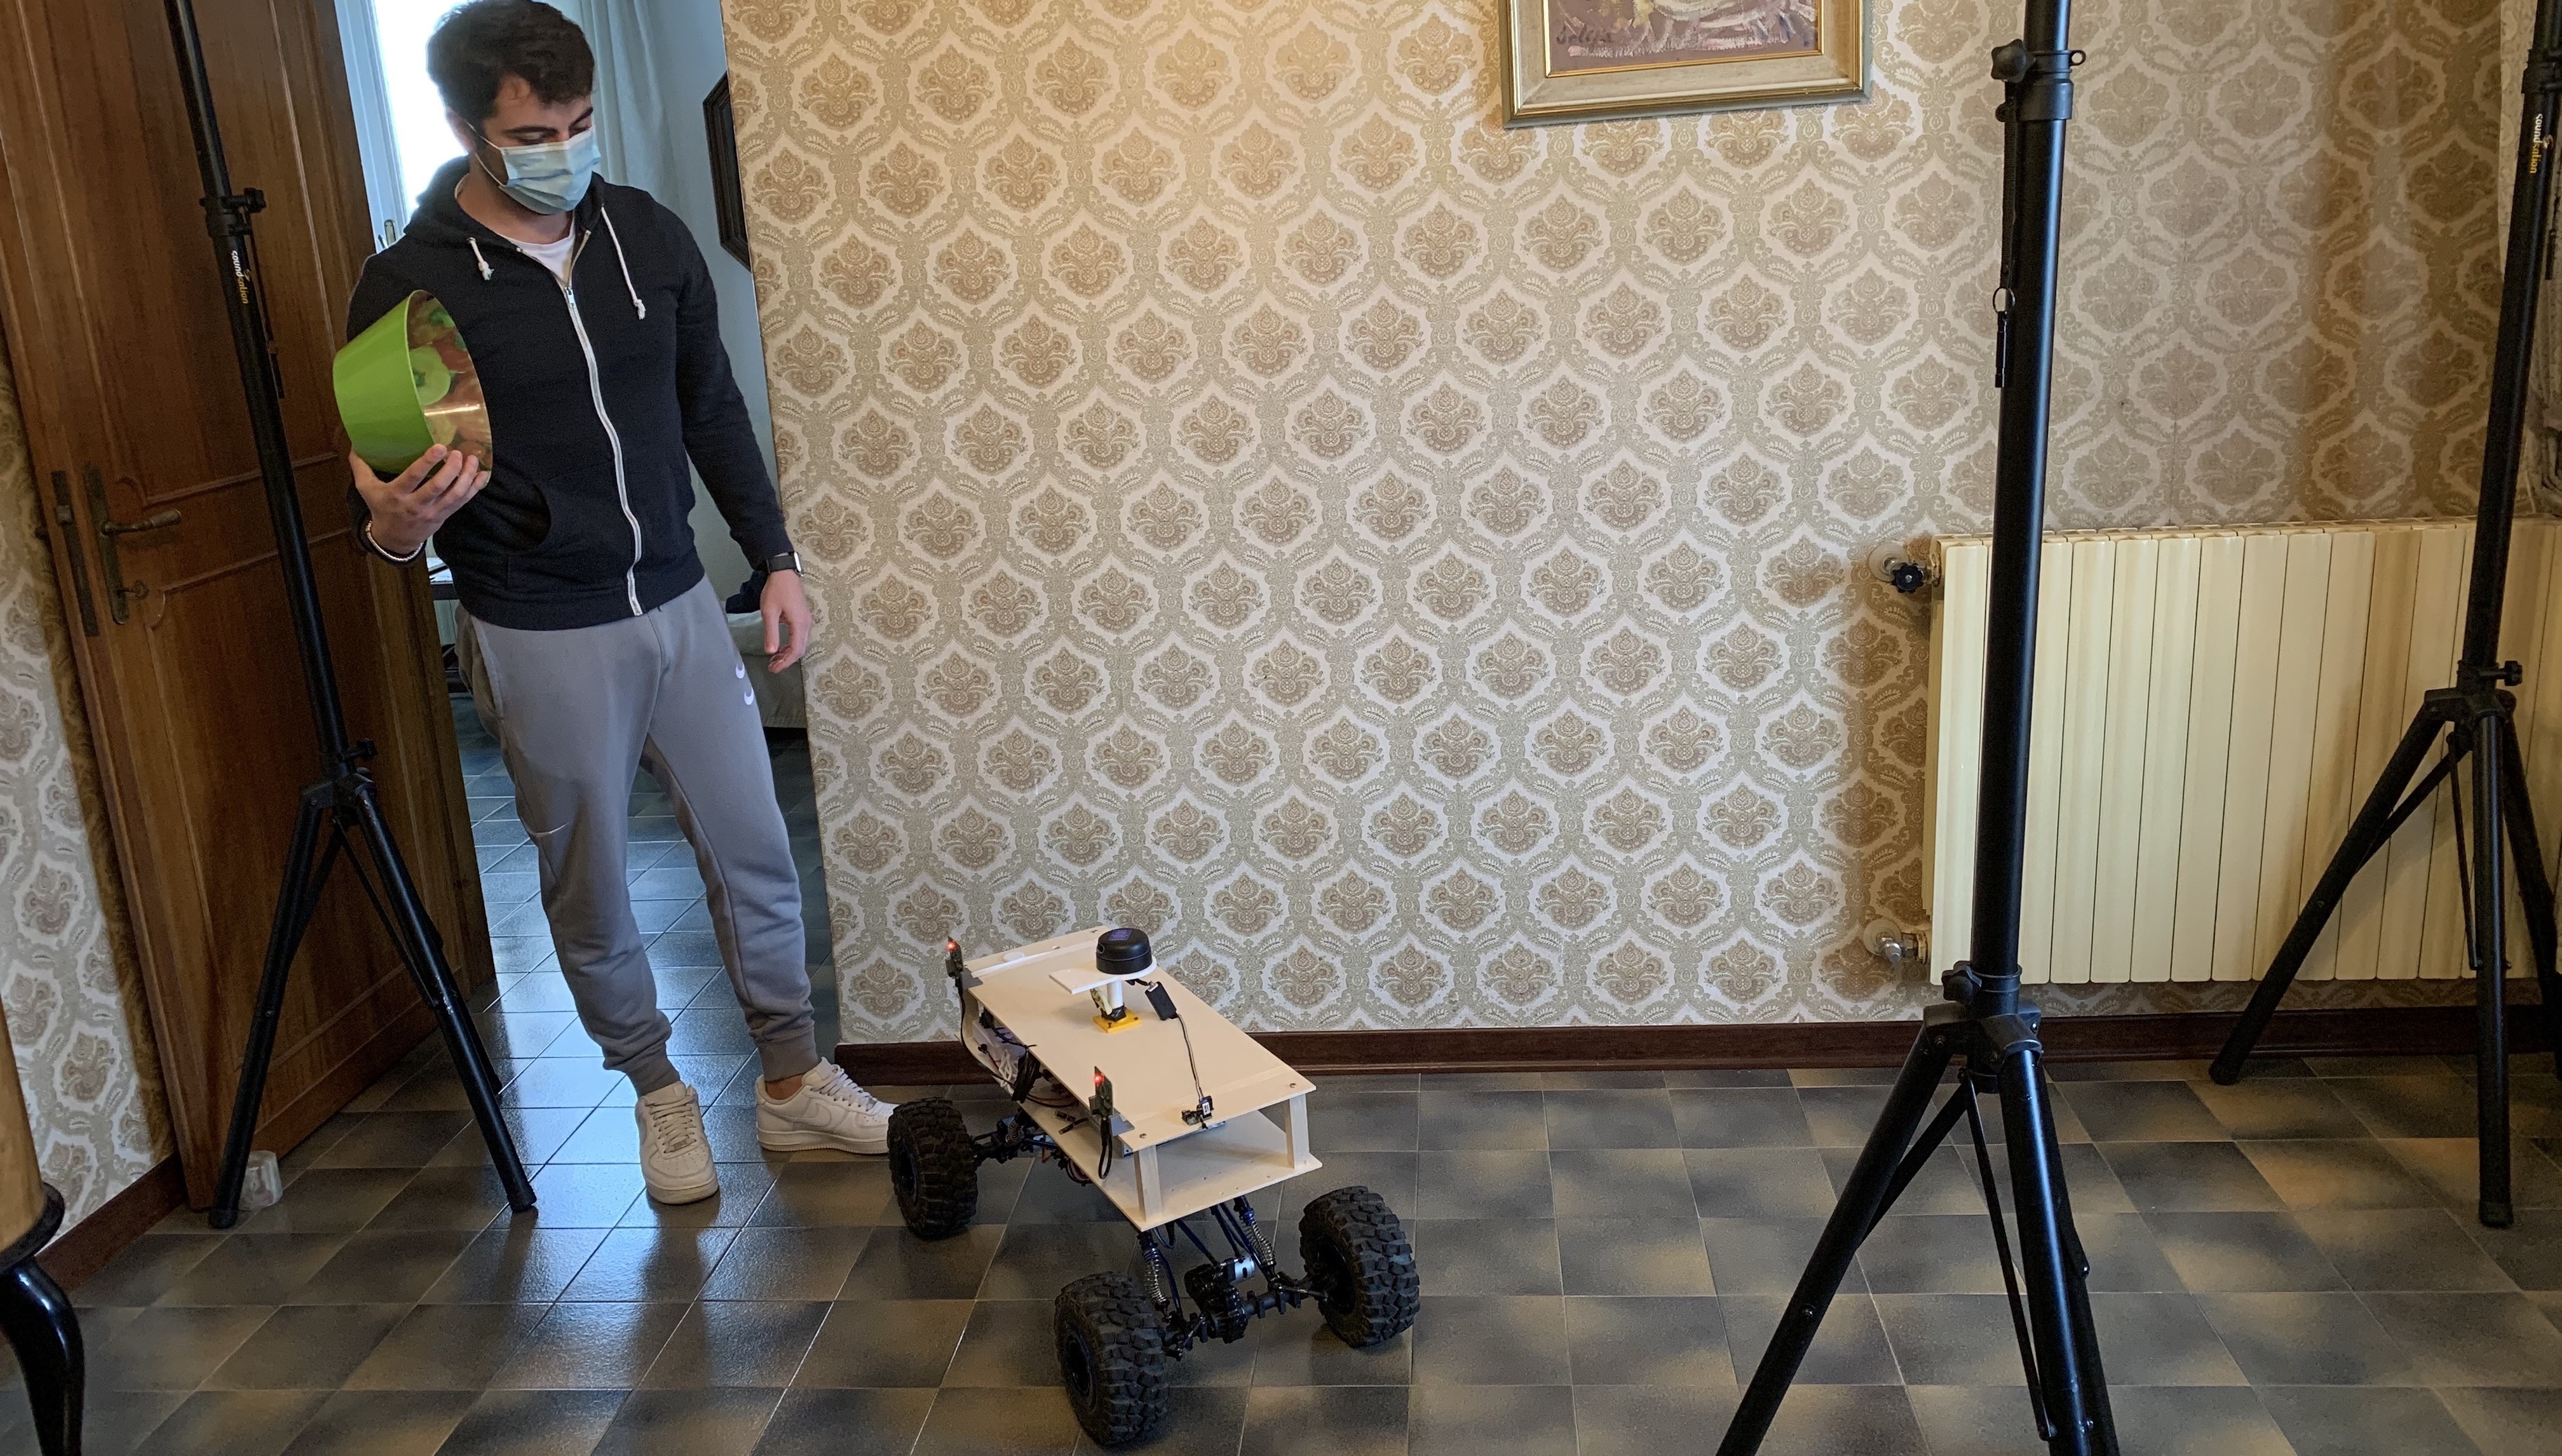
\includegraphics[width=1\linewidth]{Capitolo3/Figs/esperimento3_7b.jpg}  
  \caption{Nuovamente pronto a navigare}
  \label{subfig:esp3_7b}
\end{subfigure}

\caption[Esperimento 3]{Esperimento 3}
\label{fig:esperimento_3}
\end{figure}
\clearpage

% ********************************** Sezione 3.4  **************************************
\section{Esperimento 4 - Navigazione outdoor}
\label{section3.4}
Nel quarto esperimento è stata valutata la capacità di navigazione a waypoint outdoor sfruttando solo i dati provenienti dalle UWB.

Il robot è stato gestito via \verb!ssh! inviando di volta in volta un goal ed attendendo che vi arrivasse. 

Inizialmente il setup prevedeva un posizionamento delle ancore a 20m l'una dall'altra con disposizione a quadrato, ma i risultati ottenuti non erano buoni, il segnale delle tag veniva spesso perduto ed era molto rumoroso, con errori pari anche a più di 3m.

Si è quindi passati alla disposizione indicata in (Figura~\ref{fig:uwb_axis}) dove l'asse z è posizionato diversamente; una volta effettuato questo cambiamento i risultati si sono dimostrati buoni, ottenendo quasi sempre un raggiungimento del goal, con il veicolo che si arrestava in un raggio di circa 50cm da esso, coerentemente con l'opzione selezionata a livello di controllo. I motivi dei fallimenti ottenuti sono esaminati di seguito.

\bigskip

\begin{figure}[h]
    \centering
    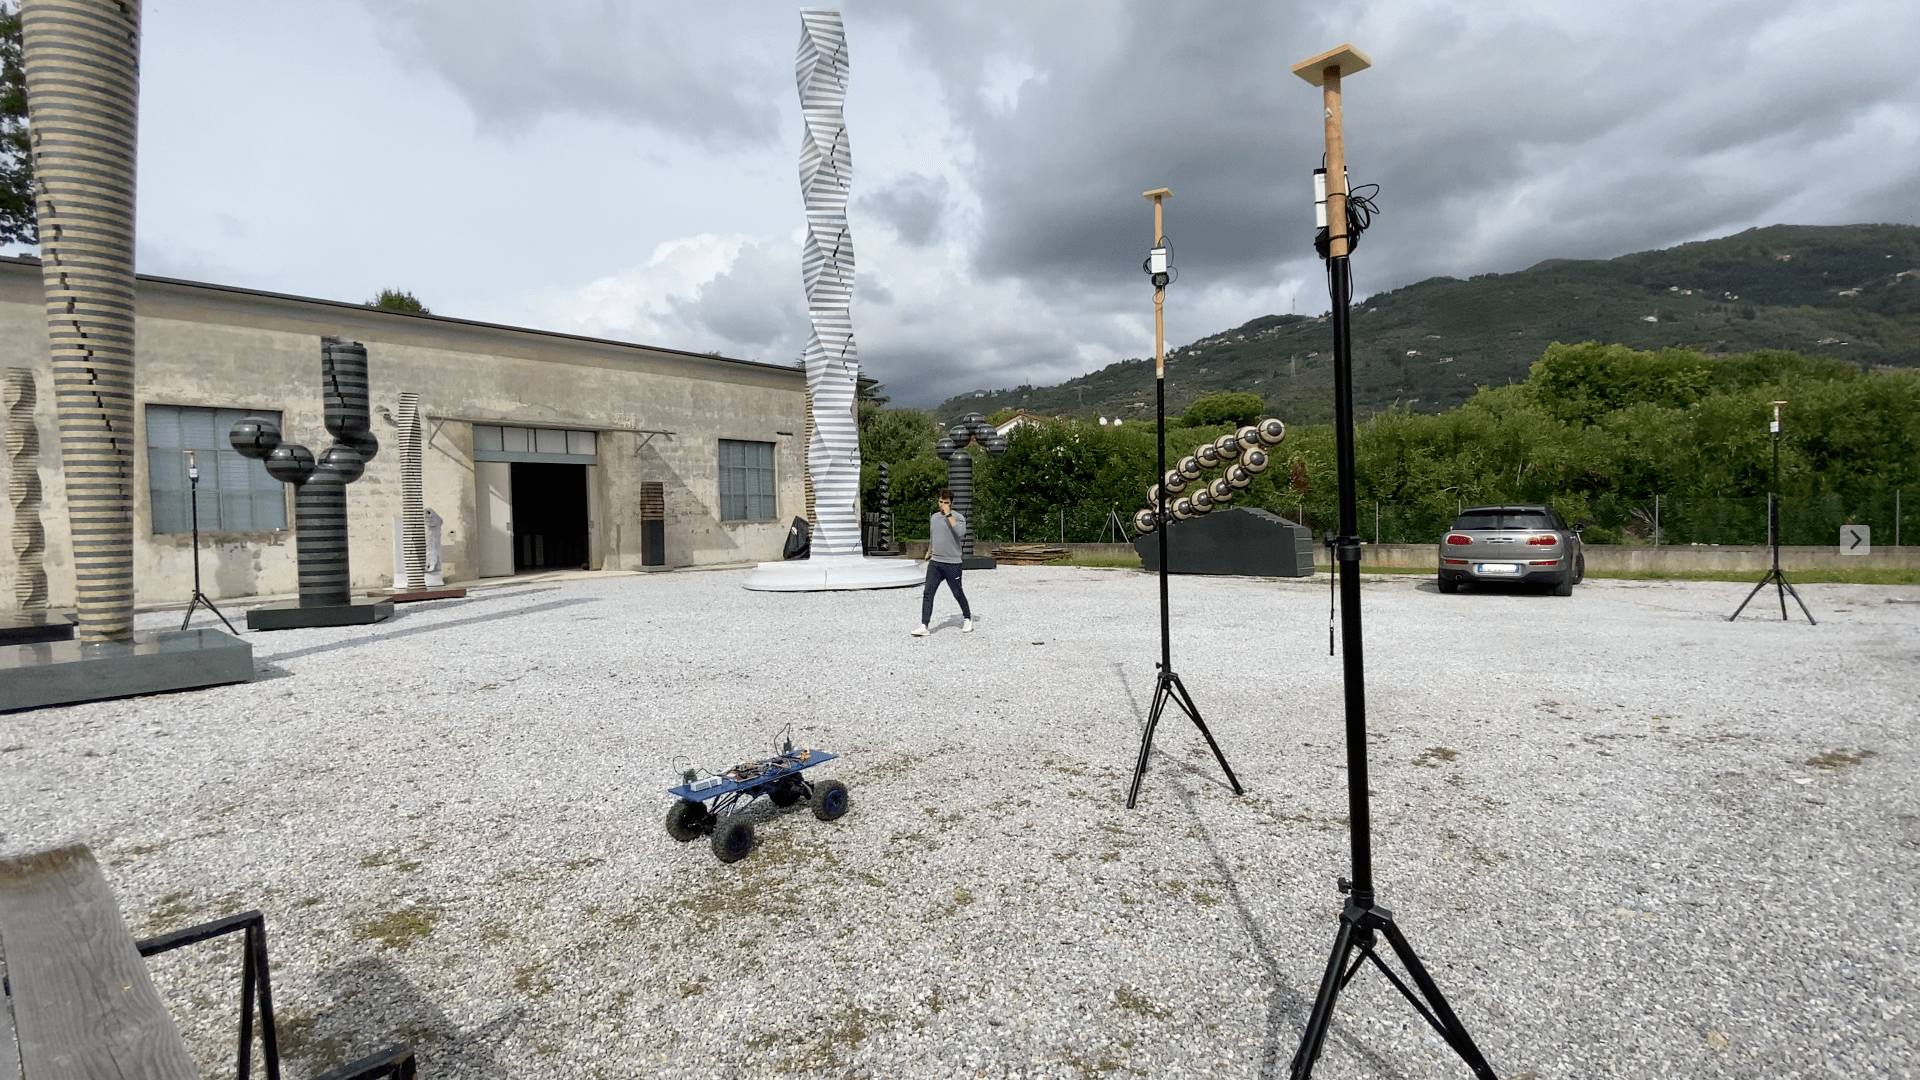
\includegraphics[width=0.95\textwidth]{Capitolo3/Figs/atelier.png}
    \caption[Posizionamento delle ancore UWB]{Posizionamento delle ancore UWB}
    \label{fig:posizione_ancore}
\end{figure}


Al variare della posizione relativa tra goal e punto di partenza, è stato possibile osservare che il controllo implementato sul robot, che non tiene conto in alcun modo della struttura dello stesso, non sempre riesce a definire una traiettoria corretta; infatti, a causa dei vincoli meccanici a cui è soggetto il veicolo, principalmente legati al raggio di sterzata, quando il goal è in una posizione difficilmente raggiungibile (ad esempio un punto interno alla circonferenza definita dal raggio di sterzo) si entra in un loop che consiste in un movimento circolare attorno ad esso. Viceversa, quando si ha un goal raggiungibile con uno spostamento rettilineo o compatibile con la capacità di sterzo del veicolo, questo non ha alcuna difficoltà a portare a termine il task.